%-------------------------------------------------------------------------------
%                            BAB IV
%               		HASIL DAN PEMBAHASAN
%-------------------------------------------------------------------------------
\fancyhf{}
\fancyfoot[C]{\thepage}
\chapter{HASIL DAN PEMBAHASAN}
\section{ANALISIS KEBUTUHAN}

Hasil dari analisis kebutuhan yang telah dilakukan adalah mendapatkan kelompok pengguna yang akan terlibat dalam penelitian dan \textit{use case diagram} untuk masing-masing pengguna. Berikut hasil analisis kebutuhan dari sistem yang dibangun.
\subsection{Kelompok Pengguna}
Kelompok pengguna dari aplikasi ini telah dapat diidentifikasikan pada tahap analisis kebutuhan pada sistem. terdapat 2 kelompok pengguna yang menggunakan aplikasi ini:
\begin{enumerate}[1.]
	\item Peneliti
	      \newline Pengguna yang menggunakan Aplikasi \textit{Mapping} berbasis Android untuk melakukan pemetaan kekuatan sinyal atau nilai RSSI dari Beacon. Aplikasi \textit{mapping} ini juga sudah memiliki sertifikat Hak Kekayaan Intelektual (HKI) dengan nomor EC00201972853.
	\item Pengguna gedung FMIPA USK
	      \newline Pengguna yang menggunakan aplikasi LocaLization di gedung Fakultas Matematika dan Ilmu Pengetahuan Alam Universitas Syiah Kuala berbasis Android.
\end{enumerate}

\subsection{Use Case Diagram}
\textit{Use case} diagram adalah diagram yang mendeskripsikan hubungan antara aktor dan sistem. \textit{Use case} diagram bisa mendeskripsikan sebuah interaksi antara satu atau lebih aktor dengan sistem yang akan dibuat. \textit{Use case} diagram juga bisa digunakan untuk mengetahui fungsi apa saja yang ada di dalam sebuah sistem dan  bisa juga mempresentasikan sebuah interaksi aktor dengan sistem. Komponen tersebut kemudian menjelaskan komunikasi antara aktor,  dengan sistem yang ada. Dengan demikian, \textit{use case} dapat dipresentasikan dengan urutan yang sederhana, dan akan mudah dipahami oleh para konsumen \citep{Yu2009}. \textit{Use Case Diagram} dari sistem yang telah dibangun dapat dilihat pada Gambar \ref{usecasemapping} dan Gambar \ref{usecasedosen}

% \begin{figure}[H]
% 	\center
% 	\shadowbox
% 	{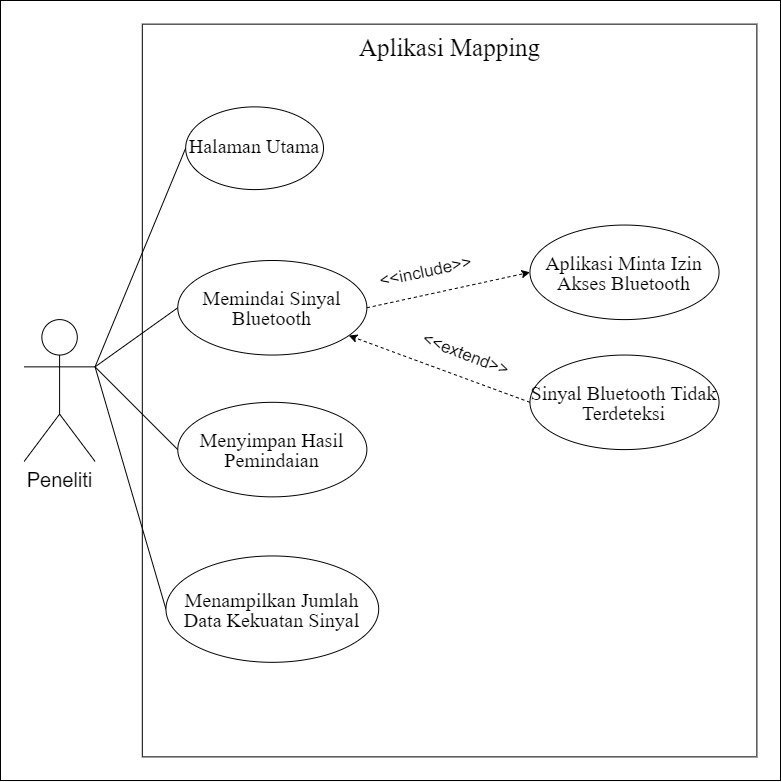
\includegraphics [width=8.5cm, height=8cm]{gambar/mapping}}
% 	\caption{\textit{Use Case Diagram} Aplikasi Mapping.}
% 	\label{usecasemapping}
% \end{figure}

\par Gambar \ref{usecasemapping} di atas menjelaskan aktivitas yang dapat dilakukan oleh peneliti saat menggunakan aplikasi \textit{mapping}. Ketika peneliti membuka aplikasi \textit{mapping}, maka akan muncul halaman beranda. Kemudian, peneliti diminta untuk mengizinkan aplikasi mengakses lokasi pada perangkat. Selanjutnya, peneliti dapat melakukan pemindaian kekuatan sinyal setelah menghidupkan Bluetooth pada perangkat \textit{smartphone}. Setelah itu, hasil dari pemindaian kekuatan sinyal tersebut disimpan di dalam server dan dapat ditampilkan jumlah data kekuatan sinyal.
\fancyhf{}
\fancyfoot[R]{\thepage}
\begin{figure}[H]
	\center
	\shadowbox
	{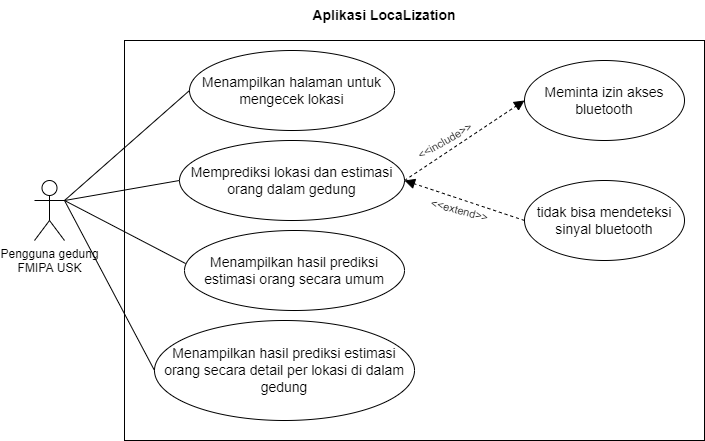
\includegraphics [width=11cm, height=7cm]{gambar/usecasediagrampenguna.drawio.png}}
	\caption{\textit{Use Case Diagram} Aplikasi LocaLization}
	\label{usecasedosen}
\end{figure}

\par Gambar \ref{usecasedosen} menjelaskan aktivitas yang dapat dilakukan oleh setiap orang yang memasuki gedung Fakultas Matematika dan Ilmu Pengetahuan Alam Universitas Syiah Kuala. Aktivitas pertama yang dapat dilakukan adalah membuka aplikasi LocaLization, pengguna dapat menikmati fitur-fitur yang tersedia seperti melihat estimasi atau jumlah orang yang sedang berada di dalam gedung, memulai proses pengecekan lokasi diri sendiri saat berada di dalam gedung FMIPA USK dengan syarat keadaan \textit{Bluetooth} pada perangkat dalam keadaan hidup dan melihat kecepatan prediksi berapa detik. Jika pengguna berada diluar gedung FMIPA USK, maka perangkat akan memprediksi pengguna sedang berada di luar jangkauan.

\begin{figure}[H]
	\center
	\shadowbox
	{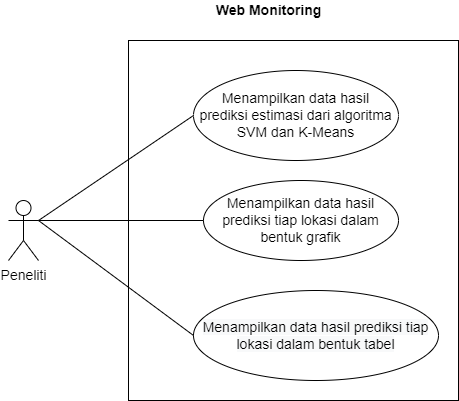
\includegraphics [width=7cm, height=6cm]{gambar/usecasediagrampeneliti.drawio.png}}
	\caption{\textit{Use Case Diagram Website Monitoring}.}
	\label{usecasewebmonitoring}
\end{figure}

Gambar \ref{usecasewebmonitoring} menerangkan tentang aktivitas yang dilakukan oleh admin atau peneliti saat  menggunakan \textit{website monitoring}. Saat peneliti atau admin membuka \textit{website monitoring}, harus \textit{login} terlebih dahulu. Setelah itu, akan langsung masuk ke halaman dasbor yang menyajikan data tentang total jumlah orang yang sedang berada di dalam gedung. Di bagian ini, akan menampilkan 2 kolom, untuk kolom pertama menampilkan data yang menggunakan algoritma SVM dan kolom kedua menampilkan data yang menggunakan algoritma K-Means. Data hasil algoritma K-Means didapatkan dari hasil penelitian rekan peneliti sebab \textit{website monitoring} ini digunakan secara bersama-sama. Kemudian di halaman lain, menampilkan data total estimasi orang yang menggunakan aplikasi ini pada tiap posisi di dalam gedung dalam bentuk tabel dan grafik.


% //TODO:Selanjutnya Buat diagram Deployment
\section{PERANCANGAN SISTEM APLIKASI LOCALIZATION}

% \subsection{Perancangan Sistem}

\par Nama LocaLization diberikan untuk nama aplikasi utama berbasis Android pada penelitian ini. Perancangan sistem adalah sekumpulan aktivitas yang mendeskripsikan secara rinci bagaimana sistem akan berjalan. Hal itu bertujuan untuk menghasilkan produk perangkat lunak yang sesuai dengan kebutuhan user. Proses ini terdiri dari dua tahap yaitu perancangan konfigurasi eksekusi sistem dalam bentuk \textit{deployment diagram} dan perancangan tampilan antarmuka (\textit{interface}).

Tahap pertama adalah merancang \textit{deployment diagram}. \textit{Deployment diagram} adalah diagram yang menjelaskan bagaimana sistem bekerja dan digunakan oleh pengguna. Berikut rancangan \textit{deployment diagram} dari sistem yang telah dibangun dapat dilihat pada Gambar \ref{deployment-diagram}.

%\begin{enumerate}
%\item \textit{Deployment Diagram} Aplikasi Mapping
\vspace{-0.2cm}
\begin{landscape}
	\begin{figure}[H]
		\center
		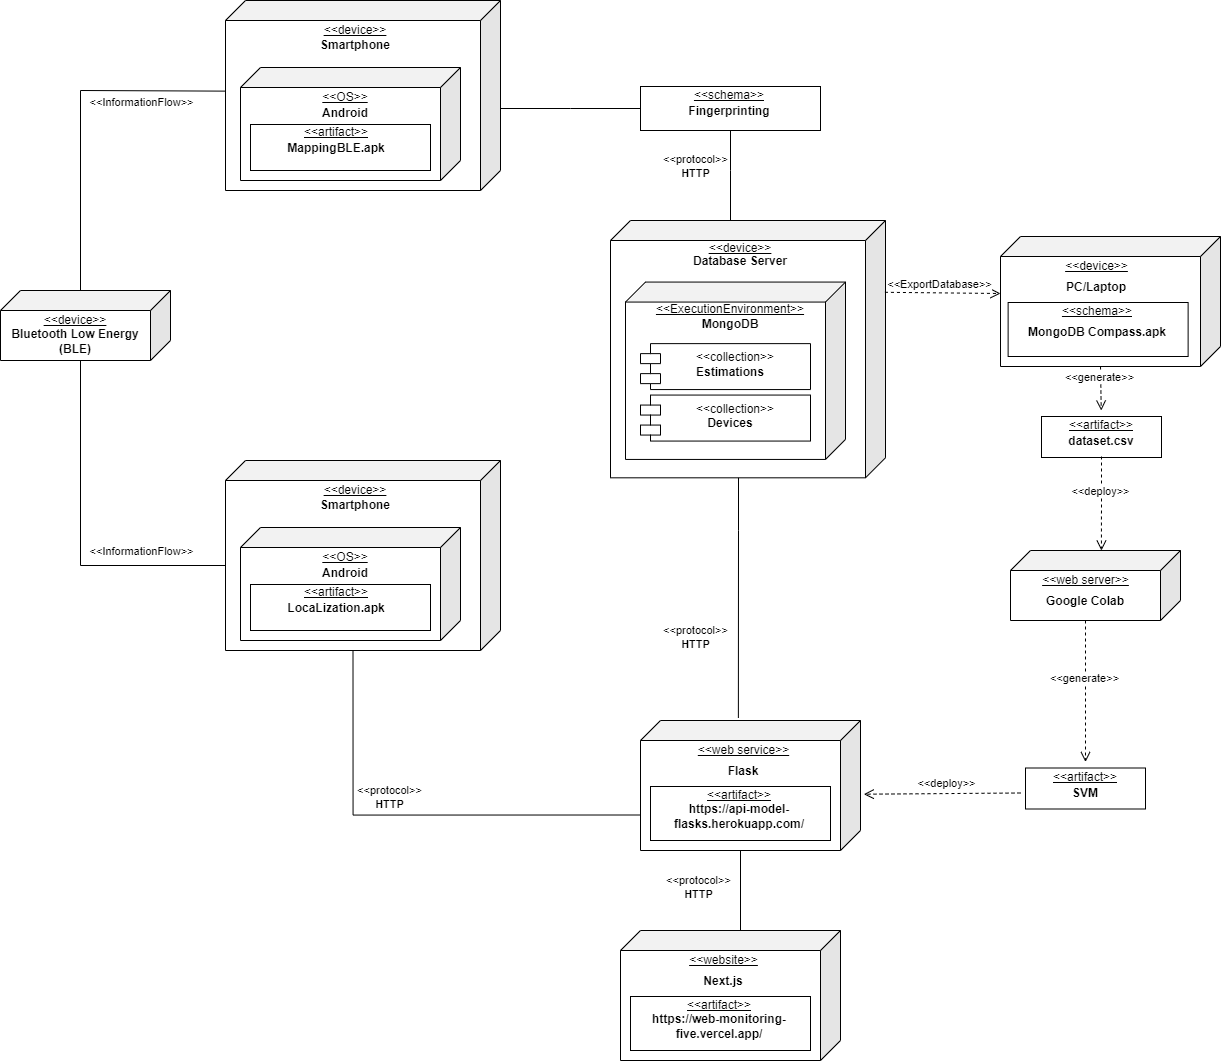
\includegraphics [width = 22.5cm, height=12cm]{gambar/diagramdeployment.png}
		\caption{Diagram \textit{Deployment}}
		\label{deployment-diagram}
	\end{figure}
\end{landscape}

Tahap kedua adalah merancang tampilan antarmuka pengguna (\textit{user interface}) sebagai mekanisme komunikasi dengan sistem. Antarmuka dari sistem yang telah dibangun adalah sebagai berikut:
\begin{enumerate}[a.]

	% \item Antar Muka Aplikasi Mapping
	%       \par Gambar \ref{aplikasimappingbagian1} menampilkan halaman awal ketika aplikasi pertama dibuka, pada halaman ini terdapat fitur untuk memasukkan nama tempat, serta fitur untuk menampilkan informasi   nama \textit{device} Bluetooth, RSSI, dan \textit{MAC address} Bluetooth, Serta pada bagian bawah terdapat empat fitur  yang masing-masing memiliki  fungsi untuk memindai , menampilkan waktu tunggu, menyimpan data dan menampilkan jumlah data yang telah disimpan. Apabila pengguna melakukan pemindaian maka akan muncul notifikasi untuk mengaktifkan Bluetooth. Apabila Bluetooth sudah hidup, maka aplikasi akan mencari nama \textit{device} Bluetooth, RSSI dan dan \textit{MAC address} Bluetooth yang ada di sekitar, pada bagian bawah fitur pemindai akan berubah menjadi stop dan fitur waktu akan menampilkan waktu tunggu  selama 10 detik, waktu ini digunakan  untuk menyamaratakan waktu pemindaian untuk setiap data. Kemudian setelah data disimpan, pada fitur yang menampilkan jumlah data yang telah disimpan yang awalnya 0 sekarang menjadi 1 yang berarti 1 data sudah dimasukkan ke dalam \textit{database server}.

	%   \vspace{-0cm}
	%   \begin{figure} [H]
	%       \begin{subfigure}{.5\textwidth}
	% 	      \centering
	% 	      % include first image
	% 	      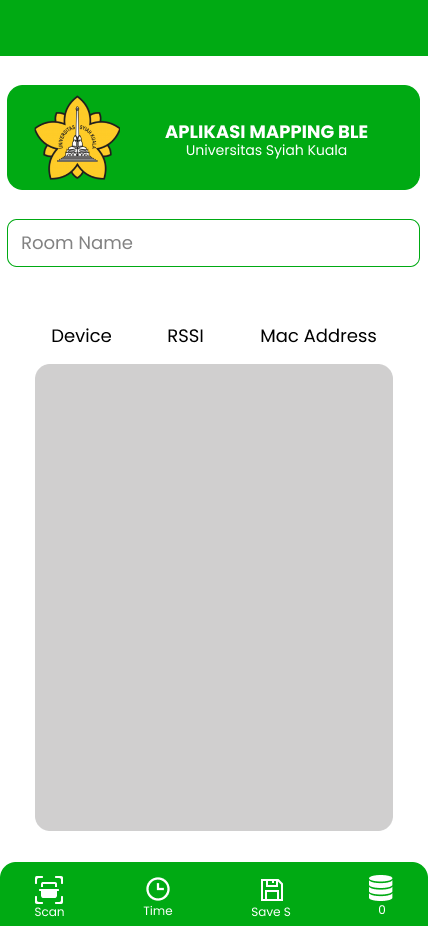
\includegraphics[width=.5\linewidth]{gambar/mapping1.png}
	% 	      \caption{Halaman awal aplikasi \textit{mapping}}
	%       \end{subfigure}
	%       \begin{subfigure}{.5\textwidth}
	% 	      \centering
	% 	      % include second image
	% 	      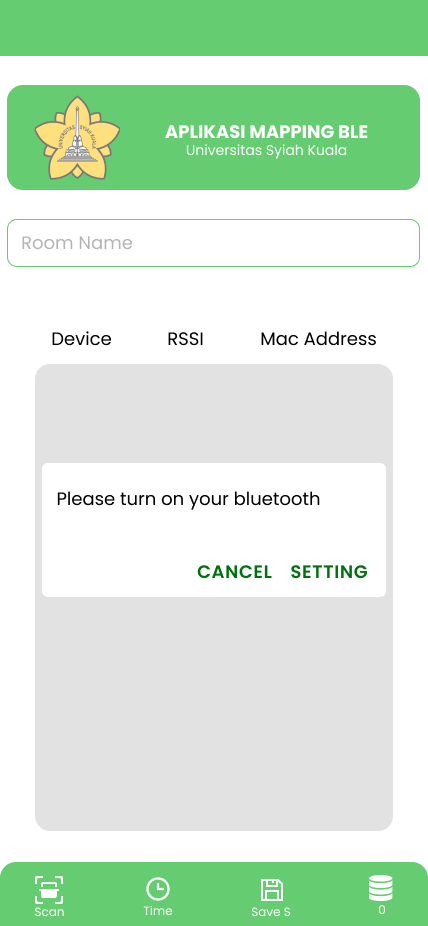
\includegraphics[width=.5\linewidth]{gambar/mapping2.png}
	% 	      \caption{Izin mengakses Bluetooth}
	%       \end{subfigure}
	%       \vspace{1cm}
	%       \newline
	%       \begin{subfigure}{.5\textwidth}
	% 	      \centering
	% 	      % include third image
	% 	      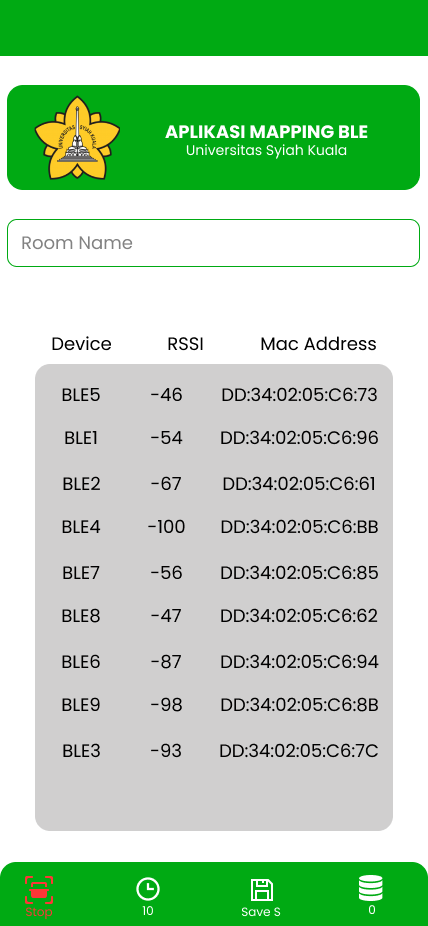
\includegraphics[width=.5\linewidth]{gambar/mapping3.png}
	% 	      \caption{Proses pemindaian kekuatan sinyal}
	%       \end{subfigure}
	%       \begin{subfigure}{.5\textwidth}
	% 	      \centering
	% 	      % include fourth image
	% 	      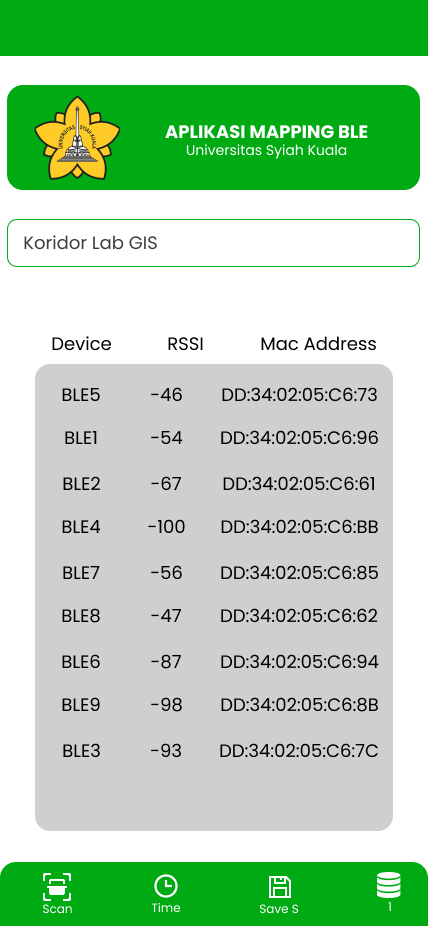
\includegraphics[width=.5\linewidth]{gambar/mapping4.png}
	% 	      \caption{Selesai proses pemindaian}
	%       \end{subfigure}
	%       \vspace{0.5cm}
	%       \caption{Tampilan Halaman Aplikasi Mapping}
	%       \label{aplikasimappingbagian1}
	%   \end{figure}

	% \vspace{1cm}
	\item AntarMuka Aplikasi LocaLization

	      \par Nama LocaLization adalah nama yang diberikan untuk aplikasi utama yang berbasis Android pada penelitian ini. Gambar \ref{aplikasiPenentuanLokasi} memperlihatkan halaman awal saat memulai menggunakan aplikasi ini. Di halaman awal setelah splash screen, pengguna akan diajak untuk menggunakan aplikasi ini agar mengetahui informasi estimasi orang dan posisi pengguna di dalam gedung. Setelah itu, akan digiring ke halaman untuk cek lokasi. Pada halaman ini, pengguna akan di minta izin untuk mengambil datanya oleh sistem agar bisa melacak keberadaannya secara anonim dan rahasia. Dengan menekan tombol Cek Lokasi, pengguna akan dianggap memberi izin jika datanya diambil untuk proses \textit{Indoor Localization System}.


	      \vspace{-0cm}
	      \begin{figure} [H]
		      \begin{subfigure}{.5\textwidth}
			      \centering
			      % include first image
			      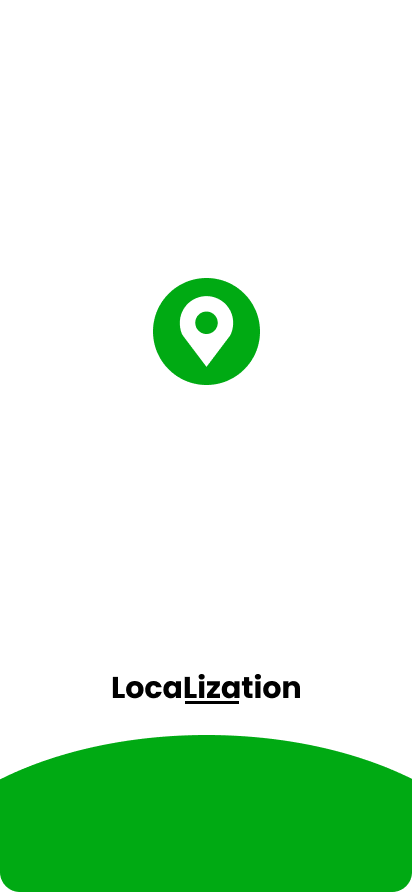
\includegraphics[width=.5\linewidth]{gambar/splashscreen.png}
			      \caption{Halaman Pertama Pembuka Aplikasi}
		      \end{subfigure}
		      \begin{subfigure}{.5\textwidth}
			      \centering
			      % include second image
			      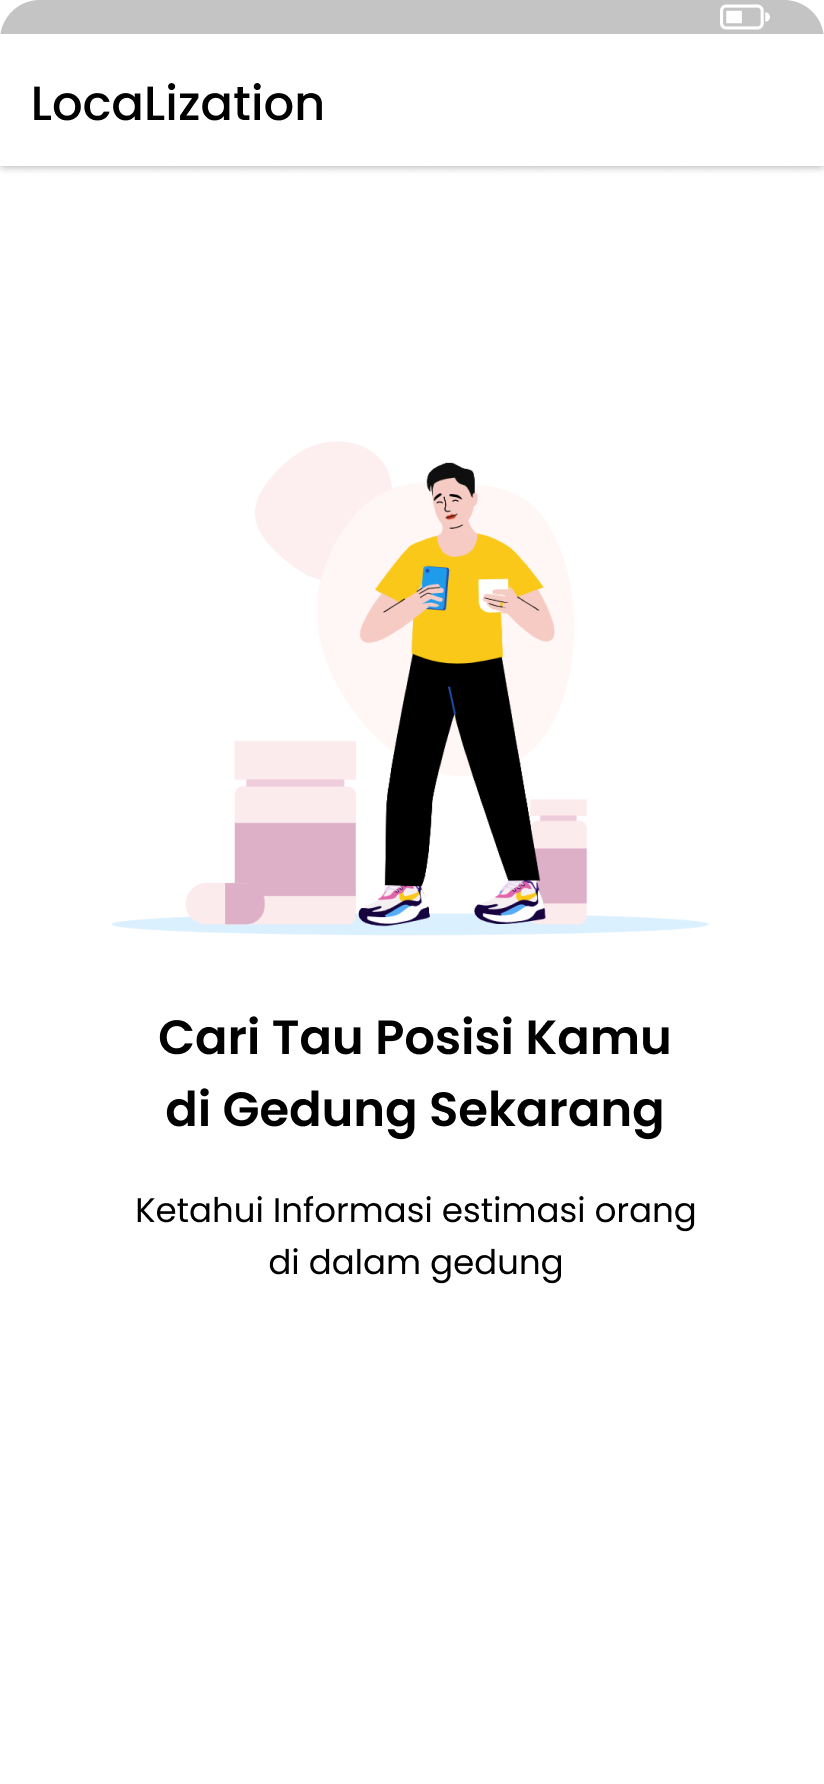
\includegraphics[width=.5\linewidth]{gambar/mulai.png}
			      \caption{Halaman Ajakan Menggunakan Aplikasi}
		      \end{subfigure}
		      \vspace{1cm}
		      \newline
		      \begin{center}
			      \begin{subfigure}{.5\textwidth}
				      \centering
				      % include third image
				      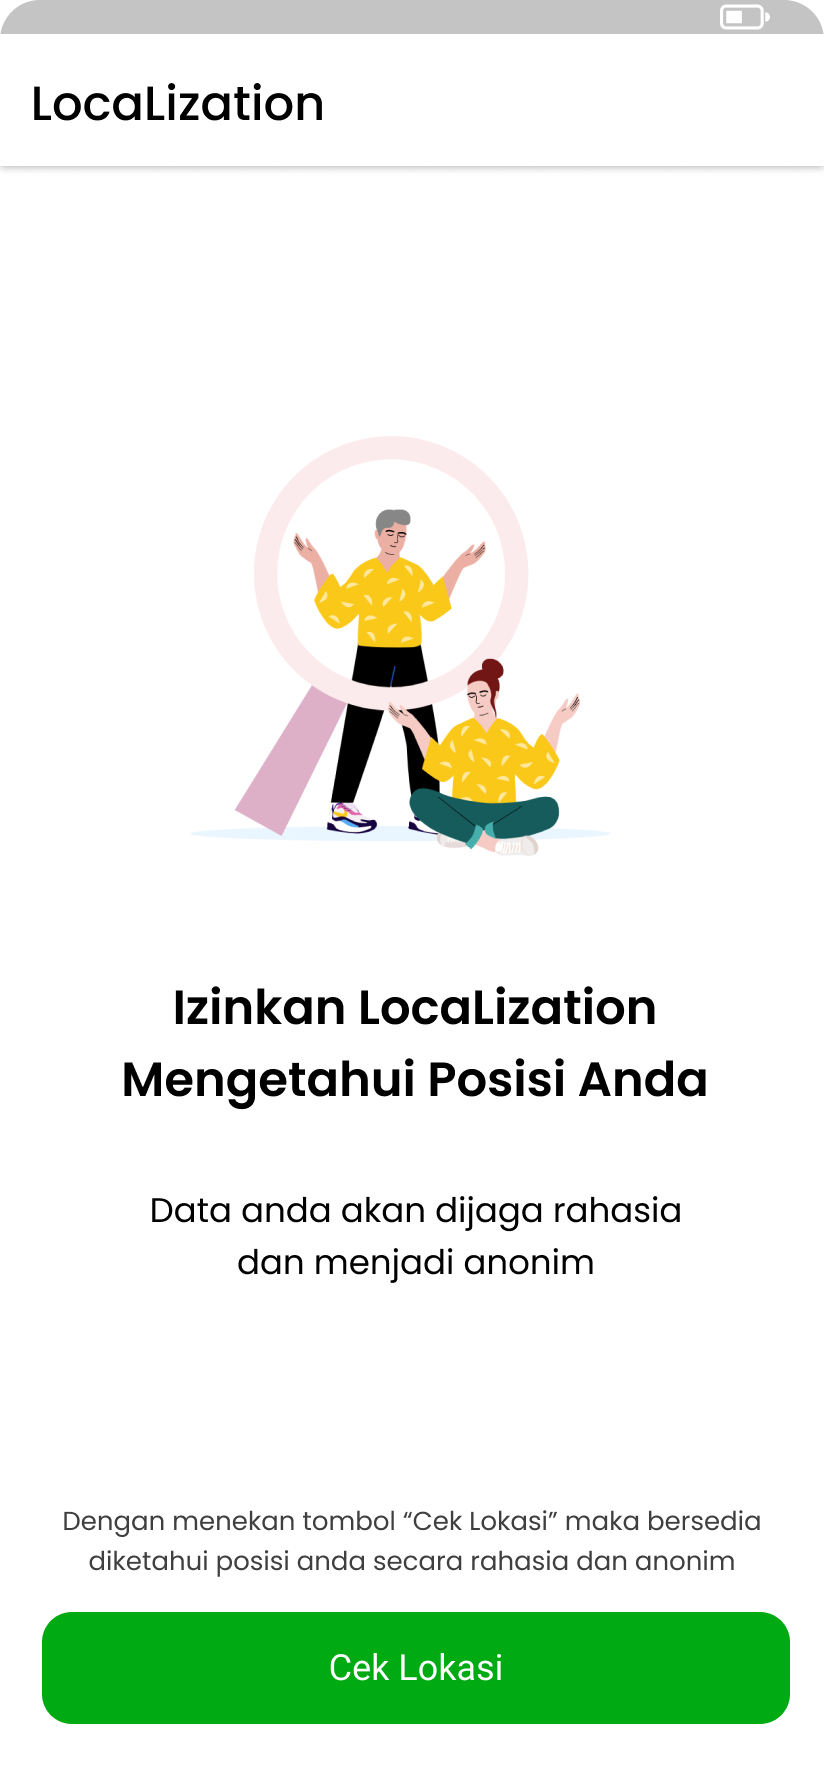
\includegraphics[width=.5\linewidth]{gambar/mulai (1).png}
				      \caption{Halaman untuk Mulai Cek Lokasi}
			      \end{subfigure}
		      \end{center}
		      \vspace{0.5cm}
		      \caption{Tampilan Awal Saat Memulai Menggunakan Aplikasi}
		      \label{aplikasiPenentuanLokasi}
	      \end{figure}

	      \vspace{0.5cm}

	      \par Proses cek lokasi memerlukan sinyal \textit{bluetooth} dan internet. Waktu yang dibutuhkan dalam \textit{scanning} adalah 10 detik. Hasil prediksi akan keluar seperti pada gambar \ref{aplikasiPenentuanLokasi2}

	      \vspace{-0cm}
	      \begin{figure} [H]
		      \begin{subfigure}{.5\textwidth}
			      \centering
			      % include first image
			      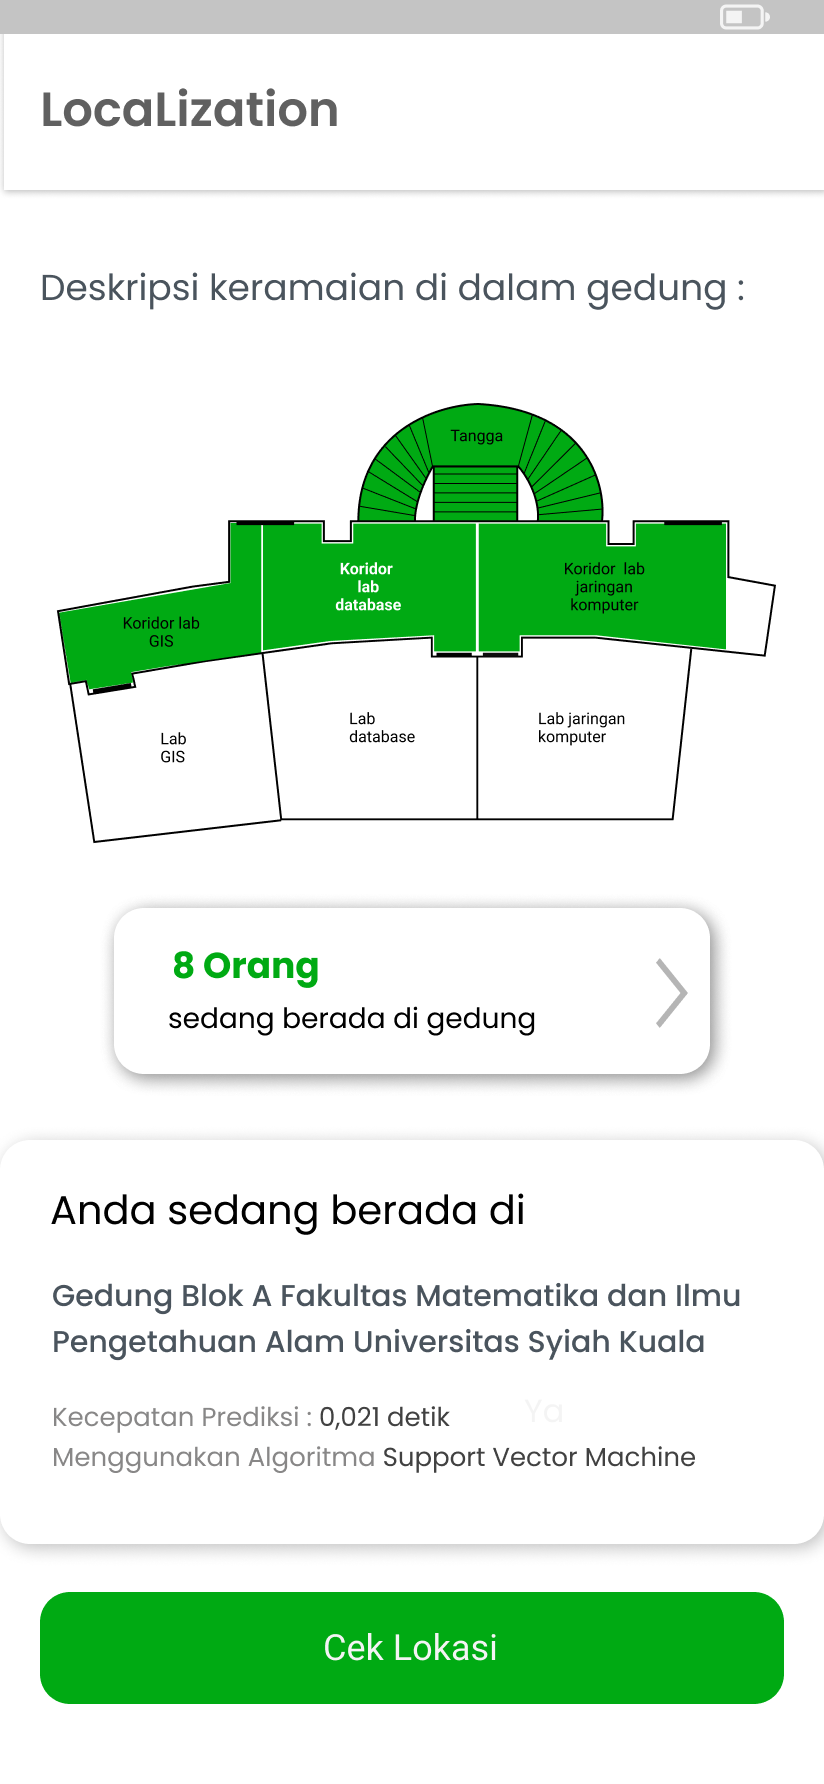
\includegraphics[width=.5\linewidth]{gambar/lantai9(1).png}
			      \caption{Halaman Pertama Pembuka Aplikasi}
		      \end{subfigure}
		      \begin{subfigure}{.5\textwidth}
			      \centering
			      % include second image
			      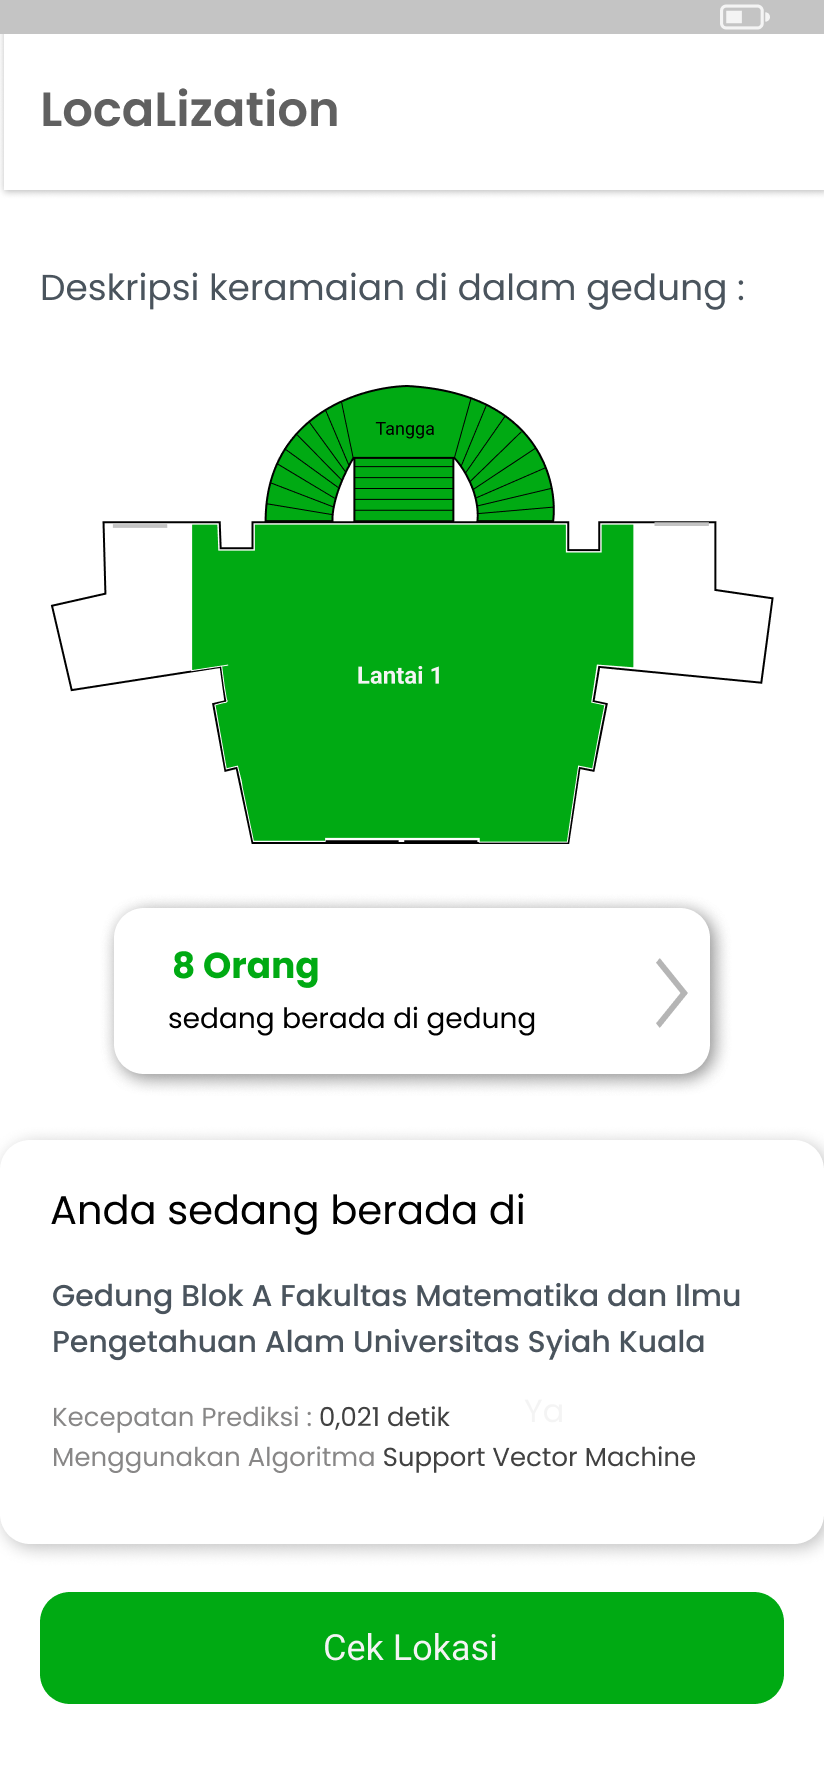
\includegraphics[width=.5\linewidth]{gambar/lantai4(1).png}
			      \caption{Halaman Ajakan Menggunakan Aplikasi}
		      \end{subfigure}
		      \vspace{1cm}
		      \newline
		      \begin{center}
			      \begin{subfigure}{.5\textwidth}
				      \centering
				      % include third image
				      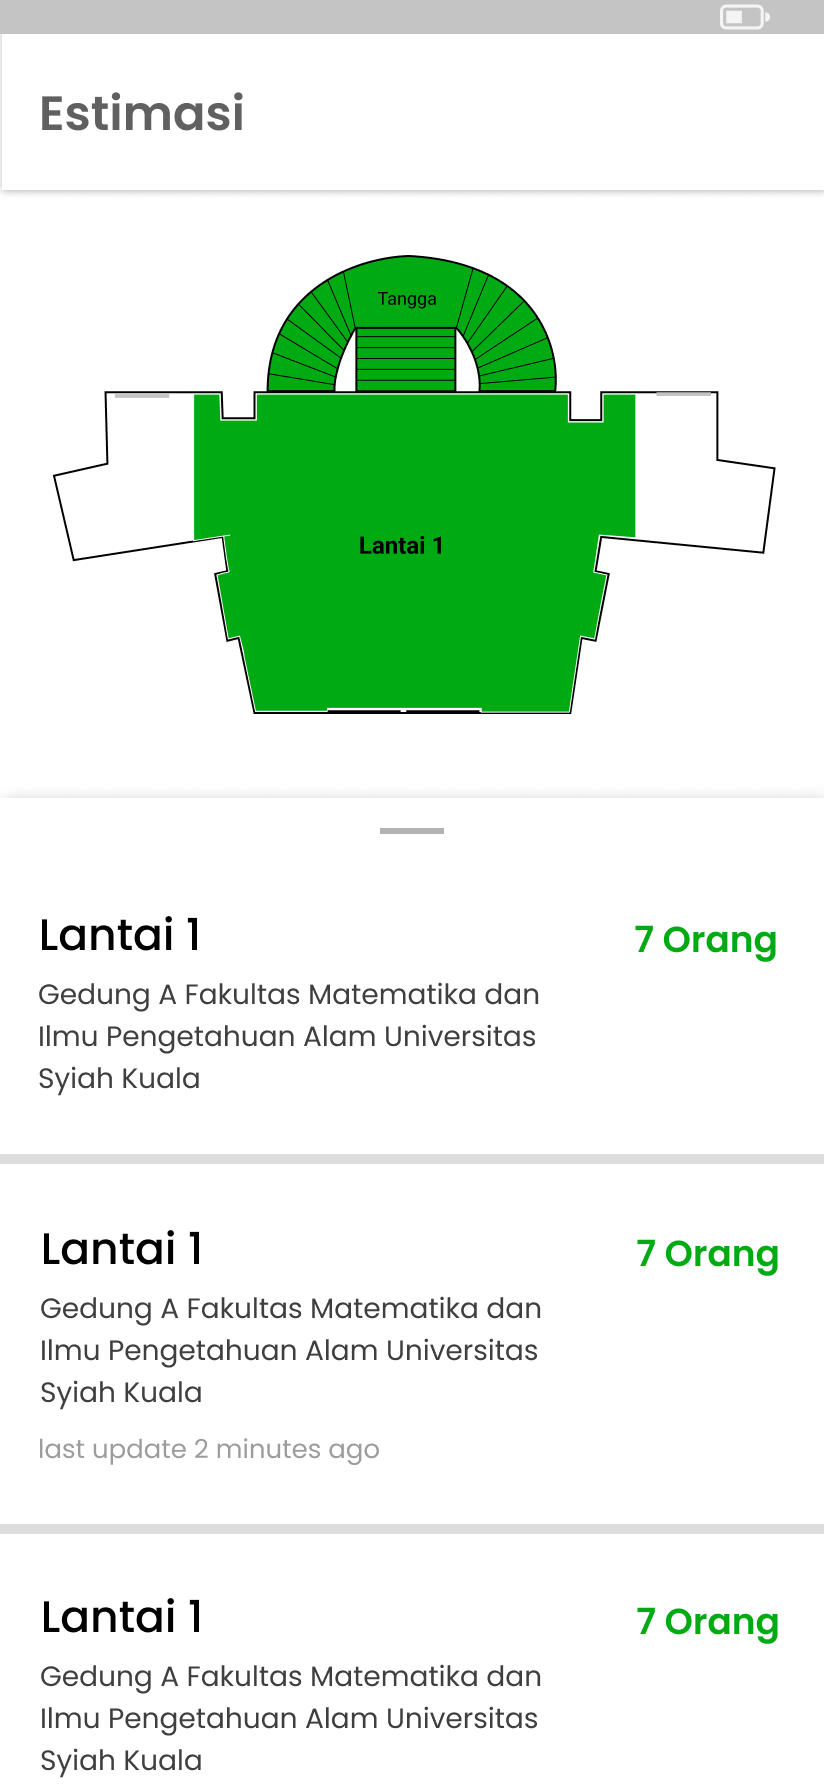
\includegraphics[width=.5\linewidth]{gambar/lantai8(1).png}
				      \caption{Halaman untuk Mulai Cek Lokasi}
			      \end{subfigure}
		      \end{center}
		      \vspace{0.5cm}
		      \caption{Tampilan Awal Saat Memulai Menggunakan Aplikasi}
		      \label{aplikasiPenentuanLokasi2}
	      \end{figure}

	      \vspace{0.5cm}

	\item AntarMuka Aplikasi \textit{Web Monitoring}

	      \par Gambar \ref{LoginWeb} adalah halaman \textit{login} untuk pengguna aplikasi \textit{web monitoring} yaitu peneliti dan admin. Setelah \textit{login}, maka peneliti atau admin langsung masuk ke halaman dasbor, seperti pada gambar \ref{Dashboard}. Pada halaman dasbor akan ditampilkan informasi data estimasi orang di dalam gedung dalam 2 kolom. Kolom pertama menampilkan data hasil dari algoritma SVM dan kolom kedua menampilkan data hasil dari algoritma K-Means yang didapatkan dari hasil penelitian rekan peneliti. Selain halaman dasbor, ada halaman yang menampilkan informasi data estimasi tiap posisi yang di dalam gedung dalam bentuk grafik dan dalam bentuk tabel. Contohnya dapat dilihat pada gambar \ref{Estimasi_Grafik} dan gambar \ref{Estimasi_Tabel}


	      \vspace{-0cm}
	      \begin{figure}[H]
		      \center
		      \includegraphics [width = 13.5 cm, height= 6.75 cm]{gambar/web/Login}
		      \caption{Halaman \textit{login Web Monitoring}}
		      \label{LoginWeb}
	      \end{figure}
	      \begin{figure}[H]
		      \center
		      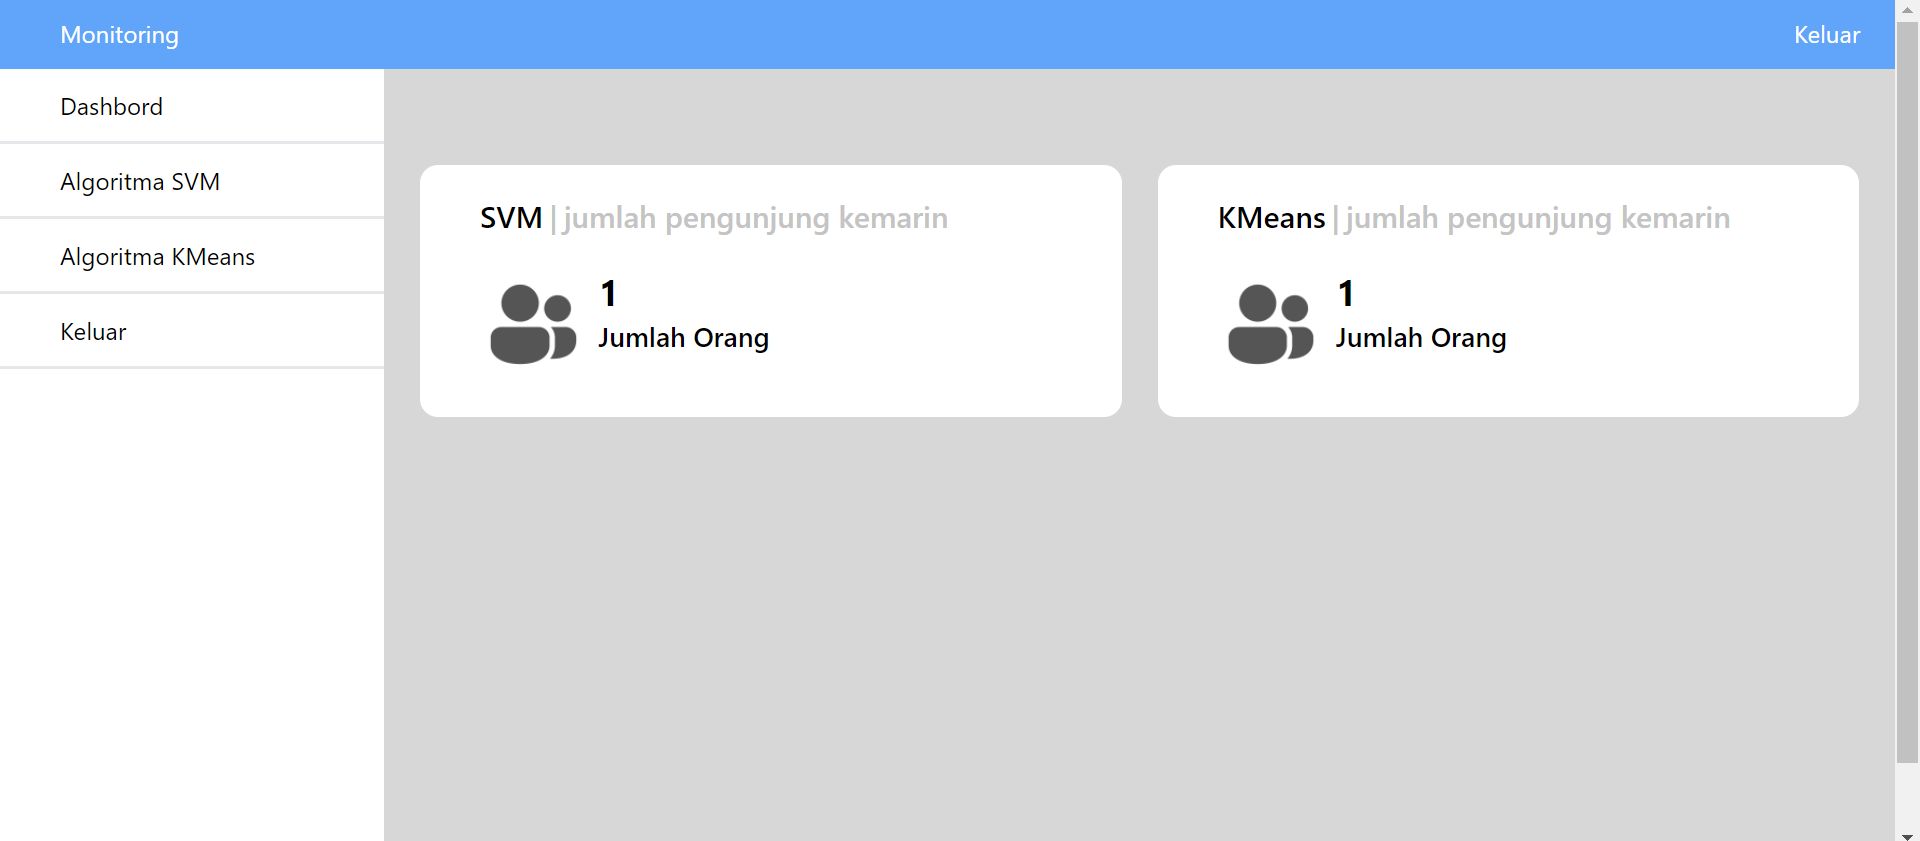
\includegraphics [width = 13.5 cm, height= 6.75 cm]{gambar/web/Dashbord}
		      \caption{Halaman \textit{dashboard}}
		      \label{Dashboard}
	      \end{figure}
	      \begin{figure}[H]
		      \center
		      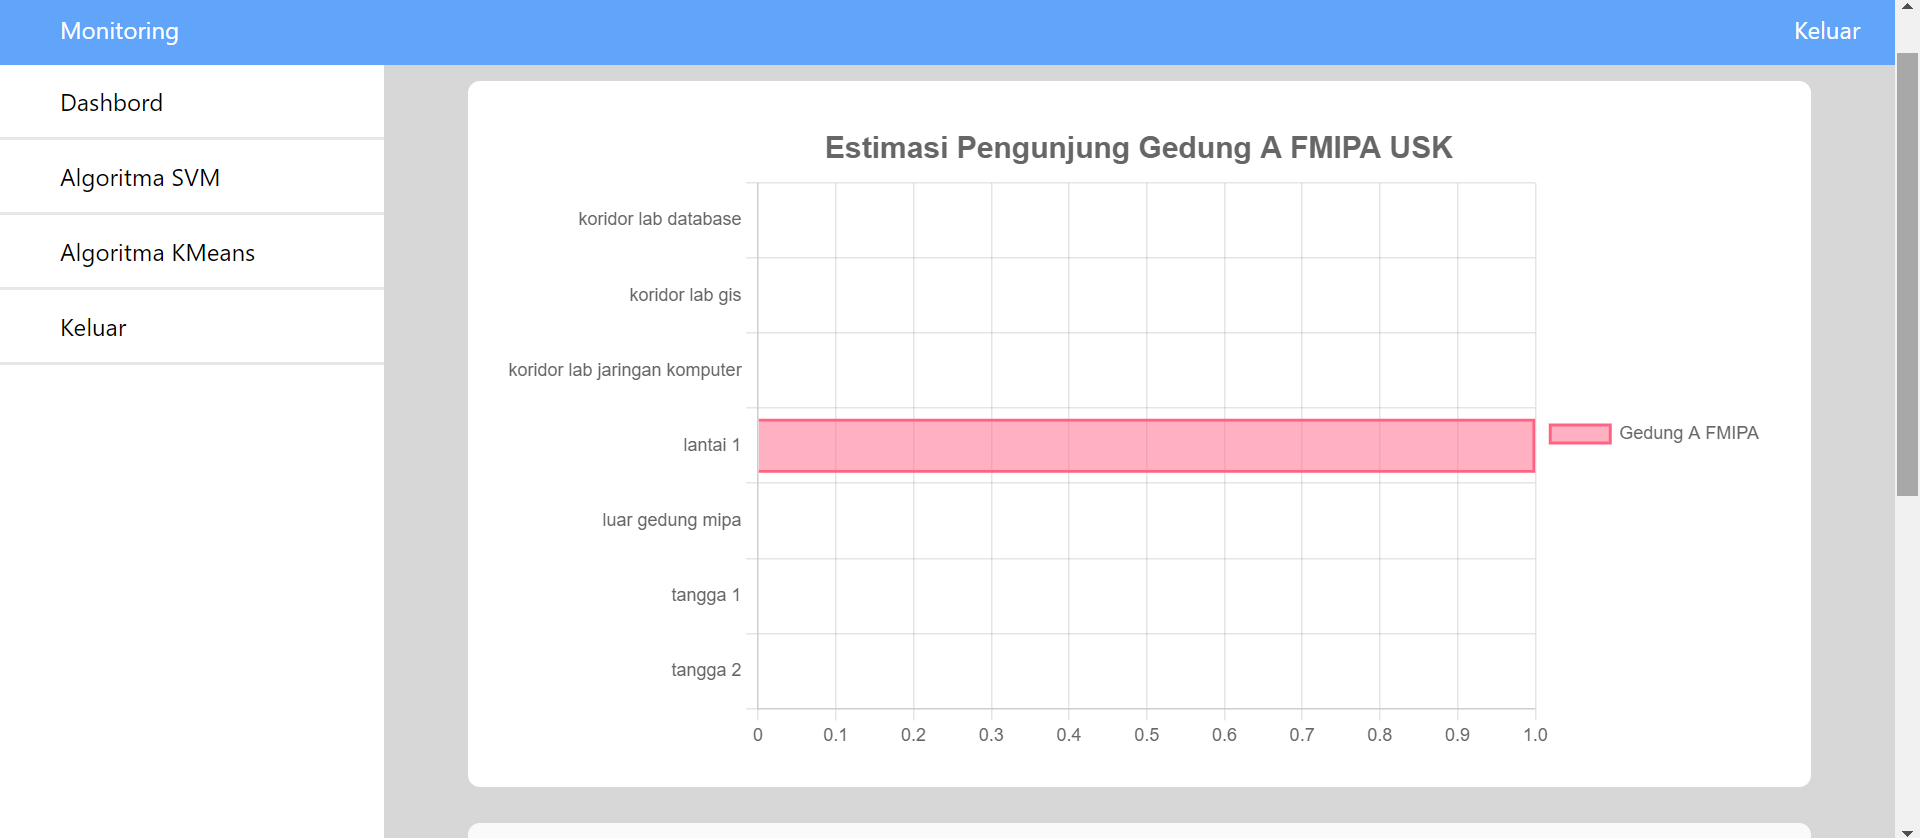
\includegraphics [width = 13.5 cm, height= 6.75 cm]{gambar/web/Estimasi_Grafik}
		      \caption{Halaman Estimasi Orang Tiap Posisi dalam Bentuk Grafik}
		      \label{Estimasi_Grafik}
	      \end{figure}
	      \begin{figure}[H]
		      \center
		      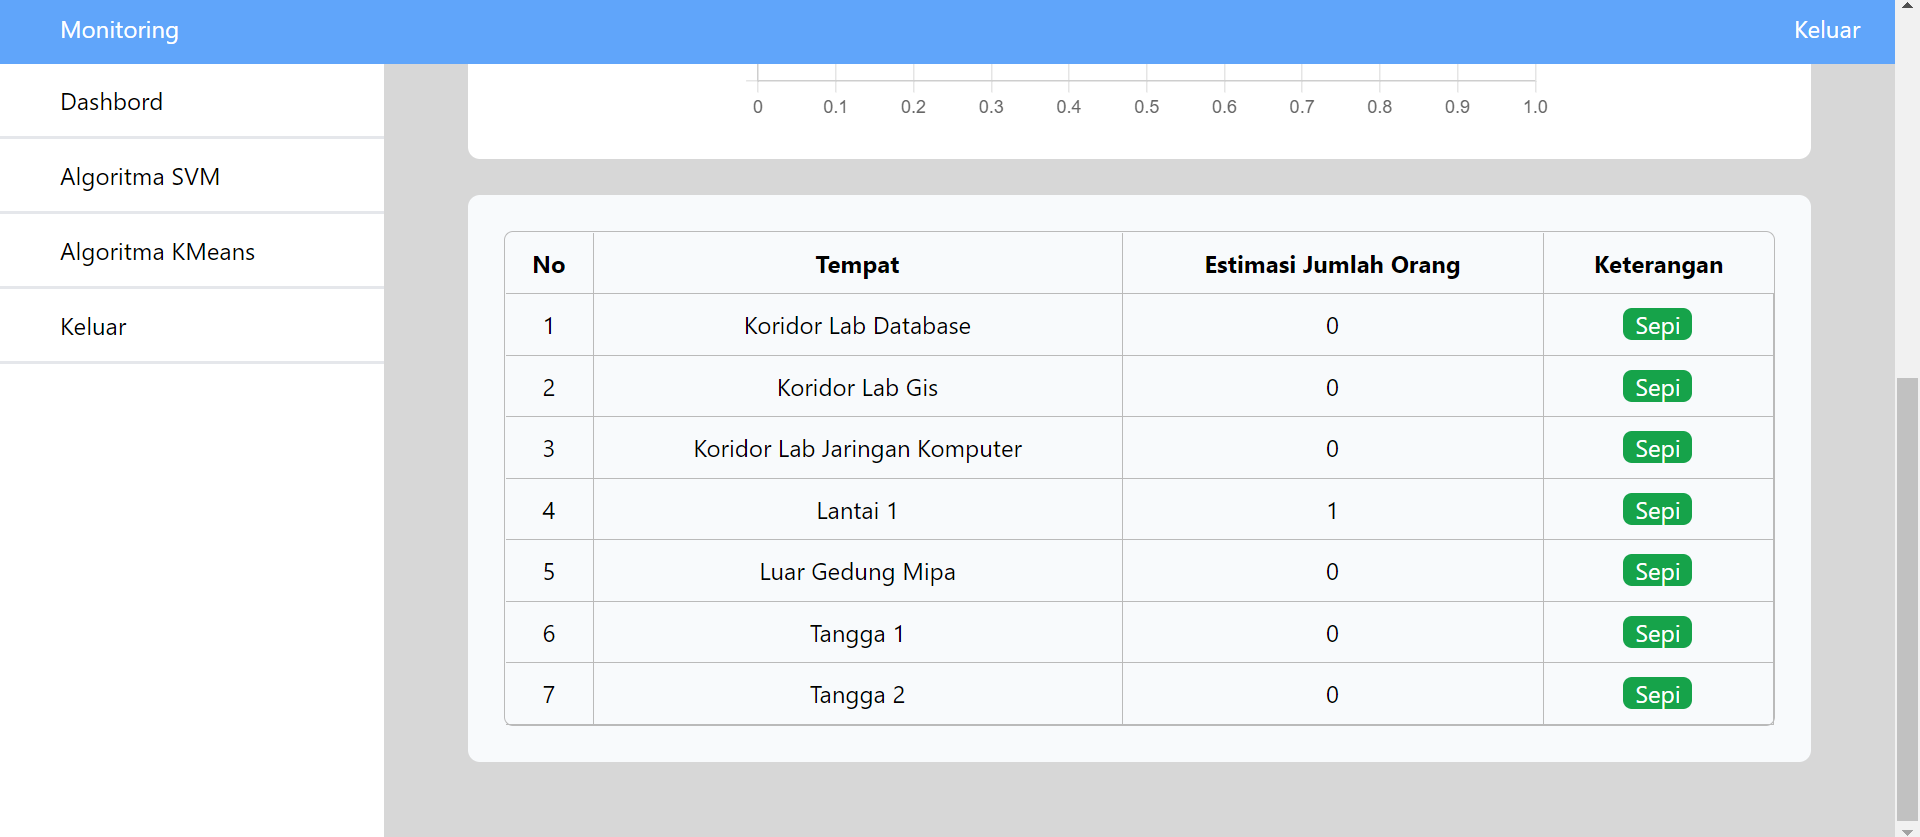
\includegraphics [width = 13.5 cm, height= 6.75 cm]{gambar/web/Estimasi_Tabel}
		      \caption{Halaman Estimasi Orang Tiap Posisi dalam Bentuk Tabel}
		      \label{Estimasi_Tabel}
	      \end{figure}
\end{enumerate}



\section{PENGUMPULAN DATA SINYAL DENGAN APLIKASI \textit{MAPPING}}
\par Proses pengumpulan data dilakukan menggunakan aplikasi pendukung yaitu aplikasi \textit{mapping}. Pada proses ini, dilakukan proses mengumpulkan data sinyal RSSI dari setiap BLE yang dipasang di setiap sudut ruangan di dalam gedung A FMIPA USK. Pada proses ini juga dibantu oleh beberapa orang dengan \textit{device} yang berbeda. Adapun daftar peserta pengumpulan data beserta \textit{device} yang digunakan dapat dilihat sebagai berikut
\begin{table}[H]
	\center
	\fontsize{10}{12}\selectfont
	\caption{Daftar Peserta Pengumpulan Data}
	\label{Daftar-Peserta-Pengumpula-Data}
	\begin{tabular}{|c|l|l|l|c|}
		\hline
		No. & \multicolumn{1}{c|}{\textbf{Nama}}                             & \multicolumn{1}{c|}{\textbf{\textit{Device} yang Digunakan}}   \\ \hline
		1.  & \begin{tabular}[c]{@{}l@{}}Indra Azari\end{tabular}            & \begin{tabular}[c]{@{}l@{}}POCO X3\end{tabular}                \\ \hline
		2.  & \begin{tabular}[c]{@{}l@{}}Aqil Fiqran Dzi'ul Haq\end{tabular} & \begin{tabular}[c]{@{}l@{}}OPPO R7SF\end{tabular}              \\ \hline
		3.  & \begin{tabular}[c]{@{}l@{}}Liza Maiyuni\end{tabular}           & \begin{tabular}[c]{@{}l@{}}SAMSUNG A30\end{tabular}            \\ \hline
		4.  & \begin{tabular}[c]{@{}l@{}}Yaumil Aghnia\end{tabular}          & \begin{tabular}[c]{@{}l@{}}SAMSUNG GALAXY A6 PLUS\end{tabular} \\ \hline
		5.  & \begin{tabular}[c]{@{}l@{}}Atika Fadhluna\end{tabular}         & \begin{tabular}[c]{@{}l@{}}XIAOMI REDMI NOTE 5\end{tabular}    \\ \hline
		6.  & \begin{tabular}[c]{@{}l@{}}Abi Farhan\end{tabular}             & \begin{tabular}[c]{@{}l@{}}XIAOMI REDMI NOTE 5\end{tabular}    \\ \hline
		7.  & \begin{tabular}[c]{@{}l@{}}Ivan Horatius\end{tabular}          & \begin{tabular}[c]{@{}l@{}}OPPO F1+\end{tabular}               \\ \hline
	\end{tabular}
\end{table}

\par Proses pengumpulan data ini menggunakan aplikasi \textit{mapping} dan wajib mengaktifkan internet dan \textit{bluetooth}. Adapun tempat yang digunakan dalam proses ini adalah gedung A FMIPA USK yaitu dari lantai 1 ke lantai 3. Proses ini dilakukan beberapa kali agar data yang didapatkan berkualitas dan jumlahnya banyak.
\par Data sinyal yang berhasil dikumpulkan adalah sebanyak 2048 baris data dengan jumlah atribut sebanyak 31 atribut dan jumlah label sebanyak 6 label. Adapun atribut pada data sinyal ini adalah data dari setiap beacon sebanyak 31 beacon dan 6 label dari masing-masing posisi di dalam gedung A FMIPA USK. 6 label pada data ini adalah lantai 1, tangga 1 (tangga yang menghubungkan lantai 1 dan 2), tangga 2 (tangga yang menghubungkan lantai 2 dan 3), koridor lab database, koridor lab GIS, dan koridor lab jaringan.

\section{PENGUJIAN AKURASI DENGAN ALGORITMA SVM}

\par Algoritma SVM dibuat dengan menggunakan kode Python dengan memanfaatkan Google Colab. Adapun langkah dalam pengujian  akurasi dengan algoritma SVM adalah sebagai berikut:

\begin{enumerate} [1.]
	\item Visualisasi Data
	      \\ Proses ini menampilkan Visualisasi data sinyal beserta labelnya. Potongan program kode Python untuk proses ini dapat dilihat pada Program 4.1 berikut ini.
	      \\
	      \begin{lstlisting}[label=MinMAxdanPCA,language=Python]
dataset = pd.read_csv("/content/drive/MyDrive/Colab Notebooks/datasets.csv",",")

bankdata = dataset.loc[:,dataTes]
# bankdata = dataset

bankdata.shape

bankdata.head()
					\end{lstlisting}
	      \captionof{lstlisting}{Potongan Kode Program Proses Visualisasi Data Klasifikasi}

	      \par Contoh tampilan visualisasi data sinyal dapat dilihat pada gambar \ref{bankdata}

	      \begin{figure}[H]
		      \centering
		      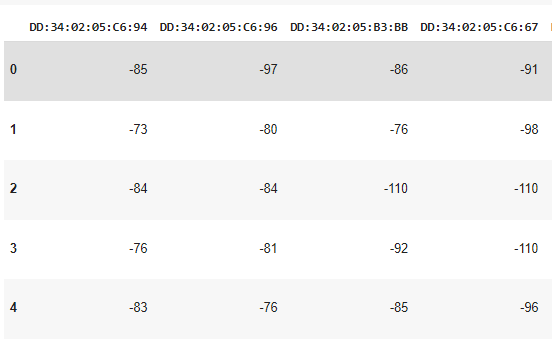
\includegraphics[width=14cm, height=9cm]{gambar/bankdata.PNG}
		      \caption{Visualisasi Data Sinyal}
		      \label{bankdata}
	      \end{figure}

	\item Pembuatan File
	      \\Proses ini akan menghasilkan file yang telah dibuat oleh \textit{library pickle} menggunakan algoritma SVM. Adapun contoh potongan kode Pythonnya seperti berikut:

	      \begin{lstlisting}[label=MinMAxdanPCA,language=Python]
import pickle
pickle.dump(svclassifier, open( "model_svm_9", "wb" ))

svclassifier = pickle.load(open( "model_svm_9", 'rb'))
		  \end{lstlisting}
	      \captionof{lstlisting}{Potongan Kode  Proses Pembuatan File Menggunakan SVM}

	      \par Untuk struktur folder dapat dilihat pada gambar

	      \begin{figure}[H]
		      \center
		      \shadowbox
		      {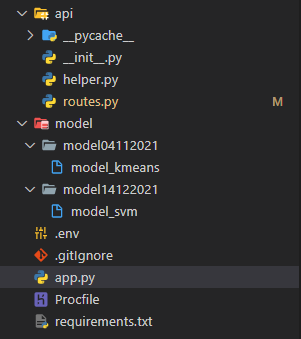
\includegraphics [width=.4\textwidth]{gambar/strukturcodemodel.png}}
		      \caption{Struktur aplikasi \textit{web service}}
		      \label{usecasemapping}
	      \end{figure}

	\item Pengujian Akurasi
	      \\ Perhitungan akurasi algoritma SVM dilakukan dengan rumus sebagai berikut:

	      \begin{equation}
		      F1-Score = \frac{2 \times Precision \times Recall}{Precision+Recall}
	      \end{equation}
	      \vspace{0.1cm}

	      \par Proses pengujian akurasi yang menggunakan kode Python dapat dilihat pada program 4.3

	      \begin{lstlisting}[label=classifier,language=Python]
from sklearn.model_selection import train_test_split
X_train, X_test, y_train, y_test = train_test_split(X, y, test_size = 0.20)

from sklearn.svm import SVC
svclassifier = SVC(kernel='linear')
svclassifier.fit(X_train, y_train)

y_pred = svclassifier.predict(X_test)

from sklearn.metrics import classification_report, confusion_matrix
print(confusion_matrix(y_test,y_pred))
print(classification_report(y_test,y_pred))
\end{lstlisting}
	      \captionof{lstlisting}{Potongan Kode Program Proses Pengujian Akurasi}
\end{enumerate}

\section{PEMBUATAN SISTEM}
\par Proses pembuatan sistem adalah tahapan implementasi dari hasil rancangan sebelumnya. Aplikasi-aplikasi yang akan dibuat adalah sebagai berikut:
\begin{enumerate}[1.]
	\item API Algoritma SVM
	      \par Bahasa pemrograman yang digunakan dalam membangun API ini adalah bahasa Python dengan menggunakan \textit{framework} Flasks.  Api ini dihubungkan dengan database MongoDb untuk menyimpan data. Api ini memiliki beberapa proses sebagai berikut:
	      \begin{enumerate}[a.]
		      \item Menyimpan file hasil algoritma SVM
		            \par Proses ini menyimpan file yang sudah dibuat sebelumnya menggunakan algoritma SVM. API mengirimkan hasil klasifikasi dari file ke aplikasi utama. Potongan program kode Python untuk proses ini dapat dilihat sebagai berikut:
		            \begin{lstlisting}[language=Python]
@app.route('/api/svm', methods=['GET', 'POST'])
@cross_origin()
def svm():
filename = 'model/model14122021/model_svm'
						
model = pickle.load(open(filename, 'rb'))
						
data = request.form.getlist('data')
if len(data) == 0:
start = time.time()
label = model.predict([[-23, -56, -110, -110, -110, -110, -110, -110, -110, -110, -110, -96,	-100,	-97,	-90,	-90,	-93,	-89,	-95,	-95, -85,	-78,	-95,	-95,	-88, -95,	-110,	-110,	-110,	-110,	-110]]).tolist()[0]
end = time.time()
return {'label': label, 'runtime': end - start}
if len(data) < 31:
return {'type': 'danger', 'message': 'data features tidak boleh dibawah 20'}
if len(data) > 31:
return {'type': 'danger', 'message': 'data features tidak boleh di atas 20'}	

start = time.time()
dataset = [int(row) for row in data]
label = model.predict([dataset]).tolist()[0]
end = time.time()
return {'label': label, 'runtime': end - start}				
								\end{lstlisting}

		      \item Menyimpan Estimasi Jumlah Orang
		            \par Pada proses ini, akan menyimpan data estimasi orang di dalam gedung A FMIPA USK. Apabila seseorang di prediksi berada di dalam gedung A FMIPA, maka akan dihitung bertambah 1 dan sebaliknya jika diprediksi berada di luar gedung A FMIPA, maka tidak dihitung ke dalam estimasi jumlah orang. Total estimasi secara keseluruhan dan detail informasi estimasi akan dikirim ke aplikasi utama yaitu aplikasi berbasis Android atau aplikasi LocaLization. Potongan kode untuk proses menambah estimasi dapat dilihat pada program 4.4 sedangkan potongan kode untuk mengurangkan estimasi orang dapat dilihat pada program 4.5.
		            \begin{lstlisting}[language=Python]
@app.route('/api/estimasi/masuk', methods=['POST'])
@cross_origin()
def masukEstimasi():
	algoritma = request.form.get('algoritma')
	label = request.form.get('label').replace(' ', '_').lower()
	currentEstimasi = db.estimations.find_one({'name': algoritma})
	now = datetime.now(pytz.timezone('Asia/Jakarta'))
	current_time = now.strftime("%m/%d/%Y, %H:%M:%S")
	if label in currentEstimasi:
		db.estimations.update_one(
			{'name': algoritma}, {'$set': {'total': currentEstimasi['total'] + 1, label: currentEstimasi[label] + 1, label+'_time': current_time, 'total_time': current_time}})
		return jsonify(algoritma=algoritma, message='Berhasil Update Data')
	db.estimations.update_one({'name': algoritma}, {
		'$set': {'total': currentEstimasi['total'] + 1, label: 1, label+'_time': current_time, 'total_time': current_time}})
	return jsonify(algoritma=algoritma, message='Berhasil Update Data')		\end{lstlisting}
		            \captionof{lstlisting}{Potongan Kode Program Proses Penambahan Estimasi}

		            \begin{lstlisting}[language=Python]
@app.route('/api/estimasi/keluar', methods=['POST'])
@cross_origin()
def keluarEstimasi():
	algoritma = request.form.get('algoritma')
	label = request.form.get('label').replace(' ', '_').lower()
	currentEstimasi = db.estimations.find_one({'name': algoritma})
	now = datetime.now(pytz.timezone('Asia/Jakarta'))
	current_time = now.strftime("%m/%d/%Y, %H:%M:%S")
	total = currentEstimasi['total'] - 1 if currentEstimasi['total'] > 0 else 0
	if label in currentEstimasi:
		countLabel = currentEstimasi[label] - \
			1 if currentEstimasi[label] > 0 else 0
		db.estimations.update_one(
			{'name': algoritma}, {'$set': {'total': total, label: countLabel, label+'_time': current_time, 'total_time': current_time}})
		return jsonify(algoritma=algoritma, message='Berhasil Update Data')
		db.estimations.update_one({'name': algoritma}, {
			'$set': {'total': currentEstimasi['total'] - 1, label: 0, label+'_time': current_time, 'total_time': current_time}})
		return jsonify(algoritma=algoritma, message='Berhasil Update Data')		\end{lstlisting}
		            \captionof{lstlisting}{Potongan Kode Program Proses Mengurangkan Estimasi}

		            Potongan kode untuk proses mengambil estimasi dari database dapat dilihat pada program 4.6.
		            \begin{lstlisting}[language=Python]
@app.route('/api/estimasi', methods=['POST'])
@cross_origin()
def getEstimasi():
		algoritma = request.form.get('algoritma')
		currentEstimasi = db.estimations.find_one({'name': algoritma})
		return jsonify(algoritma=algoritma, estimasi=parse_json(currentEstimasi))		\end{lstlisting}
		            \captionof{lstlisting}{Potongan Kode Program Proses Mengambil Jumlah Estimasi}
	      \end{enumerate}
	\item Aplikasi LocaLization
	      \par Aplikasi LocaLization adalah aplikasi utama berbasis Android. Aplikasi ini dibuat menggunakan bahasa pemrograman JavaScript dengan \textit{framework} React Native. Aplikasi ini akan memindai sinyal RSSI dari 31 beacon yang di pasang di tiap sudut ruangan selama 10 detik, kemudian data tersebut akan dikirim ke API algoritma SVM. Di dalam API ini, terdapat file hasil klasifikasi menggunakan algoritma SVM yang sudah dibuat sebelumnya. File ini menggunakan bahasa pemrograman Python. Setelah itu, API akan mengirimkan hasil klasifikasi lokasi saat ini dari file ke aplikasi utama yaitu aplikasi LocaLization. \textit{Output} yang dihasilkan adalah hasil prediksi dan informasi lainnya seperti waktu terakhir yang di\textit{update}, kecepatan data diprediksi, algoritma yang digunakan, serta informasi alamat gedung FMIPA USK.
	      \par Jika hasil prediksi adalah pengguna berada di dalam gedung, maka secara otomatis akan di tambah ke fitur estimasi orang, dan sebaliknya jika pengguna diprediksi berada di luar gedung maka tidak dihitung dan tidak dimasukkan ke dalam fitur estimasi. Adapun jika pengguna yang sudah diprediksi di dalam gedung dan masuk ke fitur estimasi lalu pengguna menekan tombol "Cek Lokasi" sekali lagi dan hasil prediksi tetap di dalam gedung A FMIPA USK, maka fitur estimasi jumlah orang tidak akan bertambah lagi, namun sebaliknya jika hasil prediksi berubah menjadi di luar gedung A FMIPA USK, maka jumlah orang pada fitur estimasi akan berkurang 1 orang. Adapun \textit{User Story} untuk aplikasi LocaLization dapat dilihat pada tabel \ref{user-story-LocaLization} sedangkan \textit{Sprint} 1 dan \textit{Sprint} 2 dapat dilihat pada tabel \ref{LocaLization-sprint-1} dan tabel \ref{LocaLization-sprint-2}.

	      \begin{table}[H]
		      \centering
		      \caption{User Story Aplikasi LocaLization}
		      \label{user-story-LocaLization}
		      \begin{tabular}{|l|l|}
			      \hline
			      Sebagai                   & \multicolumn{1}{c|}{User Story}                                                                                                      \\ \hline
			      \multirow{3}{*}{Pengguna} & Sebagai pengguna, saya dapat ikut serta sebagai sukarelawan                                                                          \\ \cline{2-2}
			                                & \begin{tabular}[c]{@{}l@{}}Sebagai pengguna, saya dapat mengetahui estimasi jumlah \\ orang di dalam gedung A FMIPA USK\end{tabular} \\ \cline{2-2}
			                                & \begin{tabular}[c]{@{}l@{}}Sebagai pengguna, saya dapat melihat denah gedung A \\ FMIPA USK\end{tabular}                             \\ \hline
		      \end{tabular}
	      \end{table}

	      \begin{table}[H]
		      \centering
		      \caption{Sprint 1 Aplikasi LocaLization}
		      \label{LocaLization-sprint-1}
		      \begin{tabular}{lllll}
			      \cline{1-2}
			      \multicolumn{1}{|c|}{\cellcolor[HTML]{FFFFFF}Item}                        & \multicolumn{1}{c|}{\cellcolor[HTML]{FFFFFF}Prioritas} &  &  & \\ \cline{1-2}
			      \multicolumn{1}{|l|}{Buat Tombol "Cek Lokasi"}                            & \multicolumn{1}{l|}{Tinggi}                            &  &  & \\ \cline{1-2}
			      \multicolumn{1}{|l|}{Buat Tampilan Cek Lokasi}                            & \multicolumn{1}{l|}{Tinggi}                            &  &  & \\ \cline{1-2}
			      \multicolumn{1}{|l|}{Mencari Lokasi Pengguna dengan API}                  & \multicolumn{1}{l|}{Sedang}                            &  &  & \\ \cline{1-2}
			      \multicolumn{1}{|l|}{Integrasi dengan React-Native-ble-plx}               & \multicolumn{1}{l|}{Tinggi}                            &  &  & \\ \cline{1-2}
			      \multicolumn{1}{|l|}{Buat Tampilan Estimasi}                              & \multicolumn{1}{l|}{Sedang}                            &  &  & \\ \cline{1-2}
			      \multicolumn{1}{|l|}{Buat List Lokasi dan Keterangan Jumlah Orang}        & \multicolumn{1}{l|}{Sedang}                            &  &  & \\ \cline{1-2}
			      \multicolumn{1}{|l|}{Buat tombol kembali untuk ke halaman denah}          & \multicolumn{1}{l|}{Sedang}                            &  &  & \\ \cline{1-2}
			      \multicolumn{1}{|l|}{Buat Tampilan denah Gedung A FMIPA}                  & \multicolumn{1}{l|}{Tinggi}                            &  &  & \\ \cline{1-2}
			      \multicolumn{1}{|l|}{Buat Tampilan di Luar Gedung A FMIPA}                & \multicolumn{1}{l|}{Tinggi}                            &  &  & \\ \cline{1-2}
			      \multicolumn{1}{|l|}{Buat tombol untuk melihat detail dari setiap lokasi} & \multicolumn{1}{l|}{Sedang}                            &  &  & \\ \cline{1-2}
		      \end{tabular}
	      \end{table}

	      \begin{table}[H]
		      \centering
		      \caption{Sprint 2 Aplikasi LocaLization}
		      \label{LocaLization-sprint-2}
		      \begin{tabular}{|l|l|}
			      \hline
			      \rowcolor[HTML]{FFFFFF}
			      \multicolumn{1}{|c|}{\cellcolor[HTML]{FFFFFF}Item}            & \multicolumn{1}{c|}{\cellcolor[HTML]{FFFFFF}Prioritas} \\ \hline
			      Add Async Storage                                             & Tinggi                                                 \\ \hline
			      Ambil data estimasi jumlah orang menggunakan API              & Sedang                                                 \\ \hline
			      Melakukan integrasi pewarnaan terhadap denah untuk keterangan & Sedang                                                 \\ \hline
			      Buat tampilan keterangan pewarnaan denah                      & Sedang                                                 \\ \hline
		      \end{tabular}
	      \end{table}

	      Potongan kode program yang terdapat dalam aplikasi ini untuk menampilkan hasil prediksi dapat dilihat pada Program berikut ini.

	      \vspace{0.4cm}
	      \lstset{language=Java,
		      basicstyle=\ttfamily\scriptsize\color{black},
		      keywordstyle=\color{javapurple}\bfseries,
		      stringstyle=\color{javared},
		      commentstyle=\color{javagreen},
		      morecomment=[s][\color{javadocblue}]{/**}{*/},
		      numbers=left,
		      numberstyle=\tiny\color{black},
		      showstringspaces=false,
		      numbersep=10pt,
		      tabsize=4,
		      showspaces=false,
		      showstringspaces=false,
		      autogobble=true,
		      xleftmargin=2em
	      }
	      \begin{lstlisting}[label=programKNNDosen]
					import axios from "axios";
					import React, { useEffect, useState } from "react";
					
					// Prediksi
					useEffect(() => {
						let formdata = new FormData();
						formdata.append("algoritma", "svm");
						setInterval(() => {
							axios
								.post(`https://api-model-flasks.herokuapp.com/api/estimasi`, formdata)
								.then((response) => {
									setEstimasi(response.data.estimasi.total);
									setSimpanLabel(response.data.estimasi);
								})
								.catch((err) => console.log(err));
						}, 1000);
				
						initBleScanner().then((data: BleDevice[] | undefined) => {
							if (data) {
								setDeviceDefaults(data);
								setDeviceTestings(data);
							}
						});
					}, []);
    \end{lstlisting}
	      \captionof{lstlisting}{Potongan Kode Program dalam aplikasi LocaLization}

	\item Aplikasi \textit{Web Monitoring}
	      \par Aplikasi \textit{Web Monitoring} dibangun menggunakan bahasa pemrograman JavaScript dan \textit{framework} Next.Js. Aplikasi ini menampilkan data estimasi orang di dalam gedung A FMIPA USK dalam bentuk kolom, tabel, dan grafik. Untuk informasi data yang menggunakan algoritma SVM dan K-Means ini akan diperbarui secara otomatis tiap beberapa detik sekali. Adapun alamat \textit{Web Monitoring} ini adalah https://web-monitoring-five.vercel.app/admin. Adapun \textit{User Story} dari \textit{Web Monitoring} dapat dilihat pada tabel \ref{user-story-web-monitoring} dan \textit{Sprint} 1 pada tabel \ref{web-monitoring-sprint-1}

	      \begin{table}[H]
		      \centering
		      \caption{User Story Website Monitoring}
		      \label{user-story-web-monitoring}
		      \begin{tabular}{|c|c|}
			      \hline
			      Sebagai                   & User Story                                                                                                                                       \\ \hline
			      \multirow{3}{*}{Peneliti} & Sebagai peneliti, Saya bisa masuk ke web monitoring                                                                                              \\ \cline{2-2}
			                                & \begin{tabular}[c]{@{}c@{}}Sebagai peneliti, Saya bisa melihat total\\ estimasi orang di dalam gedung A FMIPA USK\end{tabular}                   \\ \cline{2-2}
			                                & \begin{tabular}[c]{@{}c@{}}Sebagai peneliti, Saya bisa melihat detail estimasi orang\\ pada tiap lokasi di dalam gedung A FMIPA USK\end{tabular} \\ \hline
		      \end{tabular}
	      \end{table}

	      \begin{table}[H]
		      \centering
		      \caption{Sprint 1 \textit{Website Monitoring}}
		      \label{web-monitoring-sprint-1}
		      \begin{tabular}{|l|c|c|}
			      \hline
			      \multicolumn{1}{|c|}{\cellcolor[HTML]{FFFFFF}Item}                                                                                                        & Prioritas \\ \hline
			      \begin{tabular}[c]{@{}l@{}}Membuat fitur total estimasi jumlah orang di dalam gedung\\ menggunakan algoritma SVM\end{tabular}                             & Tinggi    \\ \hline
			      Membuat fitur login web monitoring                                                                                                                        & Tinggi    \\ \hline
			      \begin{tabular}[c]{@{}l@{}}Membuat fitur tabel yang menampilkan detail estimasi tiap \\ lokasi di dalam gedung menggunakan algoritma SVM\end{tabular}     & Tinggi    \\ \hline
			      \begin{tabular}[c]{@{}l@{}}Membuat fitur tabel yang menampilkan detail estimasi tiap \\ lokasi di dalam gedung menggunakan algoritma K-Means\end{tabular} & Tinggi    \\ \hline
			      \begin{tabular}[c]{@{}l@{}}Membuat fitur total estimasi jumlah orang di dalam gedung\\ menggunakan algoritma SVM dan K-Means\end{tabular}                 & Tinggi    \\ \hline
		      \end{tabular}
	      \end{table}
\end{enumerate}

\section{PENGUJIAN SISTEM}

\par Proses ini bertujuan untuk melihat apakah sistem yang sudah di bangun sesuai dengan rancangan. Adapun beberapa pengujian yang akan dilakukan adalah pengujian keakuratan hasil menggunakan algoritma SVM, pengujian \textit{usability} dengan menggunakan metode UMUX dan pengujian fungsionalitas menggunakan metode \textit{Black box}.

\subsection{Pengujian Keakuratan Prediksi Menggunakan Algoritma SVM}
\begin{enumerate}

	\item Pengujian Keakuratan Data Testing Menggunakan Algoritma SVM berdasarkan nilai F1-Score

	      \par Pengujian ini di analisis menggunakan kode Python. Data \textit{training} yang digunakan adalah sebanyak 1638 dan data \textit{testing} sebanyak 410 data. Pengumpulan data dilakukan dengan cara melakukan pemetaan kekuatan sinyal yang telah dijelaskan pada \textbf{BAB III}. Hasil dari proses pengujian metode klasifikasi SVM menunjukkan bahwa untuk data kekuatan sinyal memiliki rata-rata \textit{F1-Score} dengan nilai 95\%. Hasil pengujian data \textit{testing} menggunakan metode SVM ini dapat dilihat pada Tabel \ref{tabelpercobaansvm1}

	      % Please add the following required packages to your document preamble:
	      % \usepackage{multirow}
	      \begin{table}[H]
		      \center
		      \caption{Analisis Keakuratan SVM pada setiap lokasi atau label}
		      \label{tabelpercobaansvm1}
		      \begin{tabular}{|l|c|c|c|c|}
			      \hline
			      Kelas label          & \multicolumn{1}{l|}{Precision} & \multicolumn{1}{l|}{Recall} & \multicolumn{1}{l|}{F1-Score} & \multicolumn{1}{l|}{Rata-rata F1-Score} \\ \hline
			      Koridor Lab Database & 78\%                           & 92\%                        & 85\%                          & \multirow{6}{*}{95\%}                   \\ \cline{1-4}
			      Koridor Lab GIS      & 97\%                           & 87\%                        & 92\%                          &                                         \\ \cline{1-4}
			      Koridor Lab Jaringan & 92\%                           & 86\%                        & 89\%                          &                                         \\ \cline{1-4}
			      Lantai 1             & 100\%                          & 100\%                       & 100\%                         &                                         \\ \cline{1-4}
			      Tangga 1             & 99\%                           & 97\%                        & 98\%                          &                                         \\ \cline{1-4}
			      Tangga 2             & 94\%                           & 96\%                        & 95\%                          &                                         \\ \hline
		      \end{tabular}
	      \end{table}

	\item Pengujian Keakuratan Algoritma SVM Berdasarkan Penggunaan Aplikasi pada Setiap Lokasi di dalam Gedung A FMIPA USK.

	      \par Pengujian ini dilakukan bertujuan untuk menganalisis keakuratan algoritma SVM di setiap lokasi di dalam gedung A FMIPA USK. Peneliti akan menjalankan aplikasi utama berbasis Android di setiap label, masing-masing label akan diujicoba sebanyak 10 kali. Dari percobaan 10 kali pada sebuah label, maka akan dilihat berapakah yang benar diprediksi dan berapakah yang salah. Hasil dari proses pengujian metode klasifikasi SVM ini menunjukkan hasil sebesar 86,67\%.  Hasil pengujian menggunakan metode SVM pada setiap label ini dapat dilihat pada Tabel \ref{tabelpercobaansvm2}

	      % Please add the following required packages to your document preamble:
	      % \usepackage{multirow}
	      % \usepackage[table,xcdraw]{xcolor}
	      % If you use beamer only pass "xcolor=table" option, i.e. \documentclass[xcolor=table]{beamer}
	      \begin{table}[H]
		      \center
		      \caption{Analisis Keakuratan SVM pada setiap lokasi atau label}
		      \label{tabelpercobaansvm2}
		      \begin{tabular}{|lccccccccccc|}
			      \hline
			      \multicolumn{1}{|c|}{\cellcolor[HTML]{EFEFEF}}                        & \multicolumn{11}{c|}{\cellcolor[HTML]{EFEFEF}Percobaan}                                                                                                                                                                                                                                                   \\ \cline{2-12}
			      \multicolumn{1}{|c|}{\multirow{-2}{*}{\cellcolor[HTML]{EFEFEF}Label}} & \multicolumn{1}{c|}{1}                                  & \multicolumn{1}{c|}{2}  & \multicolumn{1}{c|}{3}  & \multicolumn{1}{c|}{4}  & \multicolumn{1}{c|}{5}  & \multicolumn{1}{c|}{6}  & \multicolumn{1}{c|}{7}  & \multicolumn{1}{c|}{8}  & \multicolumn{1}{c|}{9}  & \multicolumn{1}{c|}{10} & Hasil \\ \hline
			      \multicolumn{1}{|l|}{Tangga 1}                                        & \multicolumn{1}{c|}{10}                                 & \multicolumn{1}{c|}{10} & \multicolumn{1}{c|}{10} & \multicolumn{1}{c|}{10} & \multicolumn{1}{c|}{10} & \multicolumn{1}{c|}{10} & \multicolumn{1}{c|}{10} & \multicolumn{1}{c|}{0}  & \multicolumn{1}{c|}{10} & \multicolumn{1}{c|}{10} & 90\%  \\ \hline
			      \multicolumn{1}{|l|}{Tangga 2}                                        & \multicolumn{1}{c|}{10}                                 & \multicolumn{1}{c|}{0}  & \multicolumn{1}{c|}{10} & \multicolumn{1}{c|}{0}  & \multicolumn{1}{c|}{0}  & \multicolumn{1}{c|}{10} & \multicolumn{1}{c|}{10} & \multicolumn{1}{c|}{10} & \multicolumn{1}{c|}{10} & \multicolumn{1}{c|}{10} & 70\%  \\ \hline
			      \multicolumn{1}{|l|}{Koridor Lab Jaringan}                            & \multicolumn{1}{c|}{10}                                 & \multicolumn{1}{c|}{10} & \multicolumn{1}{c|}{0}  & \multicolumn{1}{c|}{10} & \multicolumn{1}{c|}{10} & \multicolumn{1}{c|}{10} & \multicolumn{1}{c|}{10} & \multicolumn{1}{c|}{10} & \multicolumn{1}{c|}{10} & \multicolumn{1}{c|}{10} & 90\%  \\ \hline
			      \multicolumn{1}{|l|}{Koridor Lab Database}                            & \multicolumn{1}{c|}{10}                                 & \multicolumn{1}{c|}{10} & \multicolumn{1}{c|}{10} & \multicolumn{1}{c|}{10} & \multicolumn{1}{c|}{10} & \multicolumn{1}{c|}{10} & \multicolumn{1}{c|}{10} & \multicolumn{1}{c|}{0}  & \multicolumn{1}{c|}{0}  & \multicolumn{1}{c|}{10} & 80\%  \\ \hline
			      \multicolumn{1}{|l|}{Koridor Lab GIS}                                 & \multicolumn{1}{c|}{10}                                 & \multicolumn{1}{c|}{10} & \multicolumn{1}{c|}{10} & \multicolumn{1}{c|}{10} & \multicolumn{1}{c|}{10} & \multicolumn{1}{c|}{10} & \multicolumn{1}{c|}{10} & \multicolumn{1}{c|}{10} & \multicolumn{1}{c|}{10} & \multicolumn{1}{c|}{10} & 100\% \\ \hline
			      \multicolumn{1}{|l|}{Lantai 1}                                        & \multicolumn{1}{c|}{10}                                 & \multicolumn{1}{c|}{10} & \multicolumn{1}{c|}{10} & \multicolumn{1}{c|}{10} & \multicolumn{1}{c|}{10} & \multicolumn{1}{c|}{10} & \multicolumn{1}{c|}{0}  & \multicolumn{1}{c|}{10} & \multicolumn{1}{c|}{10} & \multicolumn{1}{c|}{10} & 90\%  \\ \hline
			      \multicolumn{11}{|c|}{Rata-rata}                                      & 86,67\%                                                                                                                                                                                                                                                                                                   \\ \hline
		      \end{tabular}
	      \end{table}

\end{enumerate}

\subsection{Pengujian Fungsionalitas Menggunakan Black box}
\par Tujuan pengujian \textit{black box} adalah untuk menguji fungsionalitas dari aplikasi yang telah dibuat dengan cara menjalankan aplikasi tersebut apakah sesuai dengan alur bisnis yang diinginkan atau tidak. Proses ini melihat fungsi yang tidak sesuai pada aplikasi dan kesalahan-kesalahan aplikasi dalam mengerjakan suatu perintah. Pengujian \textit{black box} dilakukan pada aplikasi utama berbasis Android yaitu aplikasi LocaLization dan aplikasi \textit{web monitoring}. Beberapa fitur aplikasi yang diuji menggunakan metode \textit{black box} dapat dilihat pada Tabel \ref{blackbox-aplikasi-utama}, dan Tabel \ref{blackbox-web-monitoring}

%BLACKBOX APLIKASI LocaLization%

\begin{table}[H]
	\center
	\caption{Pengujian \textit{Black box} Aplikasi LocaLization}
	\label{blackbox-aplikasi-utama}
	\begin{tabular}{|c|l|l|l|l|}
		\hline
		\multicolumn{1}{|l|}{No} & Nama Pengujian                                                                     & Skenario                                                                                               & Tampilan                                                                                                        & Hasil    \\ \hline
		1                        & \begin{tabular}[c]{@{}l@{}}Menghidupkan \\ bluetooth\end{tabular}                  & \begin{tabular}[c]{@{}l@{}}Tekan "allow"\\ pada notifikasi\\ yang muncul\end{tabular}                  & Bluetooth akan aktif                                                                                            & Berhasil \\ \hline
		2                        & \begin{tabular}[c]{@{}l@{}}Lakukan proses\\ pemindaian \\ sinyal BLE\end{tabular}  & \begin{tabular}[c]{@{}l@{}}Tekan tombol \\ "cek lokasi" \\ saat berada di \\ dalam gedung\end{tabular} & \begin{tabular}[c]{@{}l@{}}Diarahkan ke halaman\\ denah gedung\end{tabular}                                     & Berhasil \\ \hline
		3                        & \begin{tabular}[c]{@{}l@{}}Lakukan proses\\ pemindaian \\ sinyal BLE\end{tabular}  & \begin{tabular}[c]{@{}l@{}}Tekan tombol \\ "cek lokasi" \\ saat berada di \\ luar gedung\end{tabular}  & \begin{tabular}[c]{@{}l@{}}Diarahkan ke halaman\\ luar gedung\end{tabular}                                      & Berhasil \\ \hline
		4                        & \begin{tabular}[c]{@{}l@{}}Melihat denah \\ dengan keterangan\\ warna\end{tabular} & \begin{tabular}[c]{@{}l@{}}Menggeser\\ gambar denah\end{tabular}                                       & \begin{tabular}[c]{@{}l@{}}Gambar denah berwarna\\ sesuai dengan keterangan\end{tabular}                        & Berhasil \\ \hline
		5                        & \begin{tabular}[c]{@{}l@{}}Melihat detail\\ jumlah orang\end{tabular}              & \begin{tabular}[c]{@{}l@{}}Tekan tombol\\ "jumlah orang"\end{tabular}                                  & \begin{tabular}[c]{@{}l@{}}Diarahkan ke halaman\\ detail jumlah orang di\\ setiap posisi di gedung\end{tabular} & Berhasil \\ \hline
	\end{tabular}z
\end{table}

% BLACKBOX WEB Monitoring%
\begin{table}[H]
	\centering
	\caption{Pengujian \textit{Black box} Aplikasi Web Monitoring}
	\label{blackbox-web-monitoring}
	\begin{tabular}{|c|l|l|l|l|}
		\hline
		\multicolumn{1}{|l|}{No} & Nama Pengujian                                                                 & Skenario                                                                       & Tampilan                                                                                                                                     & Hasil    \\ \hline
		1                        & \begin{tabular}[c]{@{}l@{}}Melihat halaman\\ dashboard\end{tabular}            & \begin{tabular}[c]{@{}l@{}}Masuk ke halaman\\ web monitoring\end{tabular}      & \begin{tabular}[c]{@{}l@{}}Muncul halaman\\ dashboard serta total\\ pengguna yang\\ menggunakan algo-\\ ritma K-Means dan\\ SVM\end{tabular} & Berhasil \\ \hline
		2                        & \begin{tabular}[c]{@{}l@{}}Melihat detail\\ algoritma SVM\end{tabular}         & \begin{tabular}[c]{@{}l@{}}Tekan pilihan\\ "Algoritma SVM"\end{tabular}        & \begin{tabular}[c]{@{}l@{}}Muncul detail estimasi\\ pengguna algoritma \\ SVM serta keterangan\end{tabular}                                  & Berhasil \\ \hline
		3                        & \begin{tabular}[c]{@{}l@{}}Melihat detail \\ algoritma \\ K-Means\end{tabular} & \begin{tabular}[c]{@{}l@{}}Tekan pilihan\\ "Algoritma \\ K-Means"\end{tabular} & \begin{tabular}[c]{@{}l@{}}Muncul detail estimasi\\ pengguna algoritma \\ K-Means serta\\ keterangan\end{tabular}                            & Berhasil \\ \hline
	\end{tabular}
\end{table}

%AKHIR DARI TABEL%
\par Berdasarkan hasil \textit{Black box Testing} dari tabel di atas menunjukkan bahwa Aplikasi utama berbasis Android yaitu Aplikasi LocaLization dan Aplikasi Web Monitoring dapat berjalan dengan baik dibuktikan dengan  \textbf{"berhasil"} pada kolom hasil pengujian masing-masing fitur yang dikerjakan.


\begin{comment}
\bibliography{daftar-pustaka}
\end{comment}


\subsection{Pengujian \textit{Usability} Menggunakan Metode UMUX}
\par Proses pengujian ini bertujuan untuk menguji kelayakan dan kegunaan dari sistem yang telah dibuat dan akan digunakan oleh pengguna. Sebelum melakukan pengujian ini, telah dipersiapkan \textit{Test Plan} sebagai panduan pengujian yang dapat dilihat pada Tabel \ref{testplan-aplikasi-utama}.

\begin{table}[H]
	\fontsize{10}{12}\selectfont
	\center
	\caption{\textit{Test Plan} Aplikasi LocaLization}
	\label{testplan-aplikasi-utama}
	\begin{tabular}{|l|l|l|l|l|}
		\hline
		\multicolumn{5}{|c|}{\textbf{Test Plan Aplikasi LocaLization}}                                                                                                                                                                                                                                                                                                                                                                 \\ \hline
		\multicolumn{5}{|l|}{\begin{tabular}[c]{@{}l@{}}Lokasi:\\ Lantai 1 Gedung A FMIPA USK \\Lantai 3 Gedung A FMIPA USK\end{tabular}}                                                                                                                                                                                                                                                                                              \\ \hline
		\multicolumn{5}{|l|}{\begin{tabular}[c]{@{}l@{}}Skenario:\\ 1. Pengguna membuka aplikasi.\\ 2. Pengguna memahami tampilan halaman awal. \\ 3. Pengguna menekan cek lokasi di lantai 1 gedung a FMIPA USK. \\ 4. Pengguna menekan cek lokasi di lantai 3 gedung a FMIPA USK.\\ 5. Pengguna melihat hasil prediksi lokasi yang dilakukan oleh aplikasi.\\6. Pengguna melihat estimasi jumlah orang di dalam gedung\end{tabular}} \\ \hline
		\multicolumn{5}{|l|}{\begin{tabular}[c]{@{}l@{}}Alat:\\ 1. Smartphone Android\\ 2. Beacon\end{tabular}}                                                                                                                                                                                                                                                                                                                        \\ \hline
		\multicolumn{5}{|l|}{\begin{tabular}[c]{@{}l@{}}Hasil:\\ Hasil pengujian dapat dilihat pada tabel dan lampiran.\end{tabular}}                                                                                                                                                                                                                                                                                                  \\ \hline
	\end{tabular}
\end{table}

\par Pengujian UMUX dilakukan dengan memberikan kuesioner kepada responden. Isi kuesioner tersebut berisi 4 pertanyaan seperti yang sudah dibahas pada \textbf{BAB III}. Pengujian ini memiliki 23 responden. Hasil skor pengujian metode UMUX yang dilakukan dapat dilihat pada tabel \ref{UMUX} berikut.

\begin{table}[H]
	\centering
	\caption{\textit{Usability Testing} dengan menggunakan metode UMUX}
	\label{UMUX}
	\begin{tabular}{|ccccc|c|c|}
		\hline
		\rowcolor[HTML]{FFFFFF}
		\multicolumn{1}{|c|}{\cellcolor[HTML]{FFFFFF}Responden} & \multicolumn{1}{c|}{\cellcolor[HTML]{FFFFFF}\begin{tabular}[c]{@{}c@{}}Skor \\ Q1\end{tabular}} & \multicolumn{1}{c|}{\cellcolor[HTML]{FFFFFF}\begin{tabular}[c]{@{}c@{}}Skor \\ Q2\end{tabular}} & \multicolumn{1}{c|}{\cellcolor[HTML]{FFFFFF}\begin{tabular}[c]{@{}c@{}}Skor \\ Q3\end{tabular}} & \begin{tabular}[c]{@{}c@{}}Skor \\ Q4\end{tabular} & \begin{tabular}[c]{@{}c@{}}Skor \\ UMUX\end{tabular} & \begin{tabular}[c]{@{}c@{}}Skor \\ UMUX-lite\end{tabular} \\ \hline
		\multicolumn{1}{|c|}{1}                                 & \multicolumn{1}{c|}{7}                                                                          & \multicolumn{1}{c|}{1}                                                                          & \multicolumn{1}{c|}{7}                                                                          & 1                                                  & 100,00                                               & 87,90                                                     \\ \hline
		\multicolumn{1}{|c|}{2}                                 & \multicolumn{1}{c|}{7}                                                                          & \multicolumn{1}{c|}{1}                                                                          & \multicolumn{1}{c|}{7}                                                                          & 1                                                  & 100,00                                               & 87,90                                                     \\ \hline
		\multicolumn{1}{|c|}{3}                                 & \multicolumn{1}{c|}{7}                                                                          & \multicolumn{1}{c|}{2}                                                                          & \multicolumn{1}{c|}{7}                                                                          & 1                                                  & 87,50                                                & 77,06                                                     \\ \hline
		\multicolumn{1}{|c|}{4}                                 & \multicolumn{1}{c|}{6}                                                                          & \multicolumn{1}{c|}{1}                                                                          & \multicolumn{1}{c|}{7}                                                                          & 1                                                  & 95,83                                                & 82,48                                                     \\ \hline
		\multicolumn{1}{|c|}{5}                                 & \multicolumn{1}{c|}{7}                                                                          & \multicolumn{1}{c|}{1}                                                                          & \multicolumn{1}{c|}{6}                                                                          & 2                                                  & 91,67                                                & 82,48                                                     \\ \hline
		\multicolumn{1}{|c|}{6}                                 & \multicolumn{1}{c|}{6}                                                                          & \multicolumn{1}{c|}{2}                                                                          & \multicolumn{1}{c|}{6}                                                                          & 1                                                  & 87,50                                                & 77,06                                                     \\ \hline
		\multicolumn{1}{|c|}{7}                                 & \multicolumn{1}{c|}{7}                                                                          & \multicolumn{1}{c|}{1}                                                                          & \multicolumn{1}{c|}{7}                                                                          & 1                                                  & 100,00                                               & 87,90                                                     \\ \hline
		\multicolumn{1}{|c|}{8}                                 & \multicolumn{1}{c|}{7}                                                                          & \multicolumn{1}{c|}{1}                                                                          & \multicolumn{1}{c|}{6}                                                                          & 2                                                  & 91,67                                                & 82,48                                                     \\ \hline
		\multicolumn{1}{|c|}{9}                                 & \multicolumn{1}{c|}{7}                                                                          & \multicolumn{1}{c|}{1}                                                                          & \multicolumn{1}{c|}{7}                                                                          & 1                                                  & 100,00                                               & 87,9                                                      \\ \hline
		\multicolumn{1}{|c|}{10}                                & \multicolumn{1}{c|}{7}                                                                          & \multicolumn{1}{c|}{2}                                                                          & \multicolumn{1}{c|}{7}                                                                          & 2                                                  & 83,33                                                & 97,00                                                     \\ \hline
		\multicolumn{1}{|c|}{11}                                & \multicolumn{1}{c|}{7}                                                                          & \multicolumn{1}{c|}{5}                                                                          & \multicolumn{1}{c|}{7}                                                                          & 1                                                  & 83,33                                                & 87,90                                                     \\ \hline
		\multicolumn{1}{|c|}{12}                                & \multicolumn{1}{c|}{7}                                                                          & \multicolumn{1}{c|}{2}                                                                          & \multicolumn{1}{c|}{6}                                                                          & 1                                                  & 83,33                                                & 71,65                                                     \\ \hline
		\multicolumn{1}{|c|}{13}                                & \multicolumn{1}{c|}{6}                                                                          & \multicolumn{1}{c|}{2}                                                                          & \multicolumn{1}{c|}{6}                                                                          & 1                                                  & 87,50                                                & 77,06                                                     \\ \hline
		\multicolumn{1}{|c|}{14}                                & \multicolumn{1}{c|}{7}                                                                          & \multicolumn{1}{c|}{1}                                                                          & \multicolumn{1}{c|}{7}                                                                          & 2                                                  & 95,83                                                & 87,90                                                     \\ \hline
		\multicolumn{1}{|c|}{15}                                & \multicolumn{1}{c|}{7}                                                                          & \multicolumn{1}{c|}{1}                                                                          & \multicolumn{1}{c|}{7}                                                                          & 1                                                  & 100,00                                               & 87,90                                                     \\ \hline
		\multicolumn{1}{|c|}{16}                                & \multicolumn{1}{c|}{6}                                                                          & \multicolumn{1}{c|}{1}                                                                          & \multicolumn{1}{c|}{7}                                                                          & 2                                                  & 91,67                                                & 82,48                                                     \\ \hline
		\multicolumn{1}{|c|}{17}                                & \multicolumn{1}{c|}{6}                                                                          & \multicolumn{1}{c|}{1}                                                                          & \multicolumn{1}{c|}{6}                                                                          & 1                                                  & 91,67                                                & 77,06                                                     \\ \hline
		\multicolumn{1}{|c|}{18}                                & \multicolumn{1}{c|}{7}                                                                          & \multicolumn{1}{c|}{1}                                                                          & \multicolumn{1}{c|}{7}                                                                          & 1                                                  & 100,00                                               & 87,90                                                     \\ \hline
		\multicolumn{1}{|c|}{19}                                & \multicolumn{1}{c|}{7}                                                                          & \multicolumn{1}{c|}{1}                                                                          & \multicolumn{1}{c|}{6}                                                                          & 2                                                  & 83,33                                                & 71,65                                                     \\ \hline
		\multicolumn{1}{|c|}{20}                                & \multicolumn{1}{c|}{6}                                                                          & \multicolumn{1}{c|}{2}                                                                          & \multicolumn{1}{c|}{6}                                                                          & 2                                                  & 83,33                                                & 77,06                                                     \\ \hline
		\multicolumn{1}{|c|}{21}                                & \multicolumn{1}{c|}{7}                                                                          & \multicolumn{1}{c|}{1}                                                                          & \multicolumn{1}{c|}{7}                                                                          & 1                                                  & 100,00                                               & 87,90                                                     \\ \hline
		\multicolumn{1}{|c|}{22}                                & \multicolumn{1}{c|}{7}                                                                          & \multicolumn{1}{c|}{1}                                                                          & \multicolumn{1}{c|}{7}                                                                          & 1                                                  & 100,00                                               & 87,90                                                     \\ \hline
		\multicolumn{1}{|c|}{23}                                & \multicolumn{1}{c|}{6}                                                                          & \multicolumn{1}{c|}{1}                                                                          & \multicolumn{1}{c|}{6}                                                                          & 2                                                  & 87,50                                                & 77,06                                                     \\ \hline
		\multicolumn{5}{|c|}{Rata-rata}                         & 93,84                                                                                           & 84,13                                                                                                                                                                                                                                                                                                                                                                     \\ \hline
	\end{tabular}
\end{table}

\par Berdasarkan hasil pengujian \textit{usability} menggunakan metode UMUX yang telah dilakukan di atas, aplikasi LozaLization mendapat skor sebesar 93,84 sedangkan skor UMUX-lite sebesar 84,13 dengan kategori A+. Skor UMUX-lite berdasarkan \citep{Borsci2015} lebih mendekati skor SUS. Kemudian skor UMUX-lite akan dicari padanannya dengan menggunakan Gambar \ref{grafikumuxlite} dan dapat disimpulkan bahwa aplikasi LocaLization dapat diterima dengan baik, memiliki skala B, dan memiliki \textit{adjective rating excellent}.

